%% The following document is the Master's Thesis of James Kelly as produced using
%% Kile / LateX 2e. This endeavor was initially begun on 08-04-08.
%%Data collection and apparatus construction was begun in ernest in September 2007
%%Aggregates were acquired in Summer 2007

%% Last modified 11-02-08
%%

\documentclass[12pt]{article}
%for references of the author-year AAS standard
%the references are stored in a database 
%\usepackage[round,sort&compress]{natbib}
\usepackage{latexsym}
\usepackage[font=small,format=plain,labelfont=bf,up,textfont=it,up]{caption}
%The epic package allows for simple drawings to be done in line with text
%\usepackage{epic,eepic}
%pdfages allows other PDF docs to be used in this one
\usepackage[final]{pdfpages} 
%\usepackage{graphpap}
\usepackage{setspace}
\usepackage{layout}
%The geometry package allows for the margins to be set using the \geometry command
%Use either geometry or vmargin. Using both with conflict.
\usepackage{geometry}
%The vmargin package allows for the margins to be set using the \setmargins command
%\usepackage{vmargin}
\usepackage{longtable}
%In order to include graphics, a graphics package must be included
%\usepackage[dvips]{graphicx,color}
\usepackage{graphicx}
%\usepackage{epsfig}
\usepackage{floatflt}
\usepackage{amssymb,amsmath}
\usepackage{pdflscape}
\usepackage{natbib}

\geometry{letterpaper,left=1.25in,right=1in,top=1in,bottom=1in}
\doublespacing
%\setpapersize[portrait]{USletter}
%\setmarginsrb{1.25in}{1in}{1in}{1in}{0pt}{68pt}{0pt}{0mm}

%%The settings below adjust the margins manually. They are not to be used with margin
%%packages
%\setlength{\oddsidemargin}{0.25in}
%\setlength{\evensidemargin}{0.25in}
%\setlength{\topmargin}{0in}
%\setlength{\footskip}{\linewidth}
%\setlength{\paperheight}{11in}
%\setlength{\paperwidth}{8.5in}
%\setlength{\headsep}{\linewidth}
%\setlength{\textwidth}{6.25in}
%\setlength{\textheight}{9in}
\numberwithin{equation}{section} 
\numberwithin{table}{section} 
\numberwithin{figure}{section} 

\begin{document}
\pagenumbering{roman}

%uncomment this line out to produce a page displaying the margin settings
%\layout
\thispagestyle{empty}
\section*{}

%The following document generates the title page of my thesis.
%Author: James C. Gleeson
%Last Modified: 12-14-06

\doublespacing
\thispagestyle{empty}
\section*{}
\begin{center}
\textbf{AN EXPERIMENT IN BULK THERMAL SINK CAPACITIES OF UNCONSOLIDATED MATERIAL\\}
\vspace{20mm}
A Thesis\\By\\CHARLES JAMES KELLY\\
\vspace{20mm}
Submitted to the Graduate School\\Appalachian State University\\
in partial fulfillment of the requirements for the degree of\\
MASTER OF SCIENCE\\
\vspace{20mm}
\date\\
December 2008\\
Major Department: Physics and Astronomy

\end{center}
%\end{document}
%\include{Fix}
%The signature page in Latex

%Author: James Kelly
%Modified: 10-08-08

\thispagestyle{empty}
\doublespacing
\section*{}
\begin{center}
\vspace*{-18mm}
\textbf{AN EXPERIMENT IN BULK THERMAL SINK CAPACITIES OF UNCONSOLIDATED MATERIAL\\}
\vspace*{25mm}A Thesis\\by\\CHARLES JAMES KELLY\\December 2008\\
\end{center}

\vspace*{25mm}
\singlespacing
\noindent APPROVED BY:\vspace*{6mm}

\noindent
\begin{tabular}{llll}
& & &\\
& & &\\
\hline
Dr. Chris Thaxton & & &\\
Chairperson, Thesis Committee & & &\\
& & &\\
& & &\\
\hline
Dr. Adrian Daw & & &\\
Member, Thesis Committee & & &\\
& & &\\
& & &\\
\hline
Dr. T.S. Coffey & & &\\
Member, Thesis Committee & & &\\
& & &\\
& & &\\
\hline
Dr. W. Anderson & & &\\
Member, Thesis Committee & & &\\
& & &\\
& & &\\
\hline
Dr. Edelma D. Huntley\\
Dean, Research and Graduate Studies\\

\end{tabular}

\setcounter{page}{3}
%This file will be included in the ThesisMain Document as the copywright page.

%Author: James Kelly
%Last Modified: 10-08-2008

\doublespacing
\thispagestyle{empty}       %do not display page numbers
\section*{}
\begin{center}
\vspace{60mm}
Copyright \copyright  2008 by Charles James Kelly \\
All Rights Reserved.
\end{center}

\pagestyle{plain} 

%This file will be included in the ThesisMain Document as the Abstract section.
%Author: James Kelly
%Last Modified: 10-08-2008


\doublespacing
\begin{center}
\vspace{11mm}
\section{ABSTRACT}
\textbf{AN EXPERIMENT IN BULK THERMAL SINK CAPACITIES OF UNCONSOLIDATED MATERIAL}
(December 2008)\\
\vspace{6mm}Charles James Kelly, BSE Mathematics Mansfield University of Pennsylvania\\
M.S. Appalachian State University\\
Thesis Chairperson: Dr. Chris S. Thaxton\vspace{3mm}
\end{center}

Temperature analysis in upland watersheds has demonstrated that urban stormwater discharge presents significant thermal pollution concerns. High mountain streams are characteristically lower in volume and higher in flow rate variability compared to lowland creeks and rivers. These and other characteristics specific to upland streams imply a much stronger influence from discharge sources. As urban development continues to pervade mountainous regions, thermal pollution impacts on ecosystems are mounting and engineering solutions are needed. 

Construction aggregates are commonly implemented as a stormwater runoff mitigation agent to aid in sediment filtration and temperature mediation. This research is an evaluation of how specific arrangements of aggregates, such as gravel or concrete, actually affect the discharge temperatures before final release into the watershed. Aggregates are immersed in a thermally charged flow and temperature changes in the flow are recorded. Bulk energy exchange rates and quantities are then computed and compared against various aggregate characteristics. Based on the results, it appears likely that some thermal concerns can be mitigated through proper implementation of aggregate thermal sinks. It is intended that these results will contribute to a reformulation of upland construction codes to better differentiate and accommodate location specific methods of development.

%This file will be included in the ThesisMain Document as the Acknowledgements section.

%Author: James Kelly
%Last Modified: 10-08-2008

\doublespacing
\vspace{11mm}
\begin{center}
\section{ACKNOWLEDGEMENTS}
\end{center}
I wish to thank my advisor, Dr. Chris Thaxton, for serving as an irreplacable braintrust and guide in pursuing this research project, in addition to being a tireless worker who has so passionately demonstrated that the experience of his students is his top priority. Additionally, thanks are due in part to the Appalachian State University Physics Department for assistantships, equipment and funding opportunities, and to the faculty members and classmates of the same department for unending insight, excellence and guidance. Thanks to my wife Mary Dean for tolerating and feeding a graduate student, especially in the waning months of this project when it mattered the most. 



\tableofcontents
\listoffigures
\listoftables

\part*{}

%%This file will be included in the ThesisMain Document as the Experimental
%apparatus section section.

%Author: James Kelly
%Last Modified: 10-08-08

\doublespacing
\begin{center}
\section{INTRODUCTION}
\end{center}

\pagenumbering{arabic}
\subsection{Overview}
Physiographic regions are generalized as mountainous or upland based on three outstanding geological characteristics: Steep slopes, large relief and elevated bedrock. In contrast to neighboring lowland or piedmont regions, upland regions demonstrate a different set of geological behaviors, across all scales of observation. Consequently upland watersheds are decidedly unique due to their geographical location, and directly as a result of these upland characteristics, they are more sensitive to their inputs \citep{watersheds}.

Currently, urban and suburban development pervades upland regions worldwide at ever increasing rates and densities \citep{rgis}. Specific findings on upland ecological systems and overall watershed health are emerging to show developmental management practices that may be well suited for lowland regions are not effective, or perhaps more hurtful, in upland regions \citep{urban}. It is the intent of this research to further contribute to this emerging understanding regarding upland ecology, geology and impact assessment.

The research and experiments presented in this thesis were further motivated from the realization that some best management practices (BMP) and other common engineering solutions to watershed management may be ornamental, and poorly suited for an upland context \citep{urban}. Specifically, we focused on the use of construction aggregate and other unconsolidated material to thermally sink stormwater discharge at point sources. It is a common practice to fill an entrenchment intended for infiltration or local discharge with gravel, especially near waters that are sensitive to thermal charging \citep{rgis}. The gravel provides armament for the entrenchment and also is figured to thermally sink the effluent before being discharged \citep{ballast}. The discharge or surface flow interacts with the gravel in a complex and variable manner that would be difficult to measure or characterize. However, an understanding of the amount of a particular mass of aggregate could ideally sink and the rate at which the heat could be transferred could potentially offer motivations for additional solutions of thermal mitigtion or at least offer insight into the current arrangements of entrenched gravel and stream bank stabilization techniques \citep{kRocks}.

\subsection{Upland Watershed Characteristics}
Watersheds that drain upland regions are consistently dendric, high gradient waters. Using hydrogeologic definitions of order 1 being an intermittent drainage and order 5 being a large, high volume, mature river, most mountain reaches are of order 2 or less, with some prominent drainages no higher than grade 3 \citep{watersheds}. The streambeds are composed of large grains and cobbles due to intermittently large flow volumes with very high flow energies, steep profiles and elevated rates of bank erosion \citep{thaxAdd}. Due to characteristically thin soil horizons, infiltration in catchment areas is notoriously shallow, which limits baseflow causing many upper reaches to be highly intermittent, fast draining and excessively “flashy” \citep{krautBASE}. Upland waters are comparably cold, oxygen rich waters that foster a seperate ecology from lowland regions. Regional biota are, to  some degree, acclimated to frequent changes in volume and sediment load, but remain highly susceptable to large changes in water temperture \citep{urban}. Stream temperature in general serves as an excellent indicator of many upland freshwater ecosystems, because the populations are so temperature dependent. These upland waters are more sensitive to thermal inputs from all sources, such baseflow, surface heating and discharges \citep{anderson}. 

\subsection{Summary of Impacts}
Urban and suburban development fundamentally impacts these waters through variances in surface and baseflow volumes, extreme sediment loading and thermal charging, not to mention other types of explicit pollution \citep{rgis}. The sometimes shallow infilitration, and generally small aquifer size and faster baseflows that define upland hydrology are dramatically effected by dense urban development. Urban surfaces such as rooftops, streets, sidewalks and parking lots further prevent infiltration and rapidly evacuate stormwater into the nearest surface flow \citep{rgis, krautBASE}. Additionally, the installation of culverts to control flow and channelization eliminate groundwater interaction \citep{anderson}. Thermal charging occurs primarily as a result of point sources from either urban surfaces as stormwater discharge, from retention pond overflow or from industrial discharges \citep{krautBASE}.

\subsection{Boone Creek Monitoring}
Stream data are currently being collected on the Appalachian State University campus in and around Boone Creek. Boone Creek is a first-order tributary of the New River, a National Heritage River. It is typical of an upland creek, exhibiting frequent high-energy flows, a course grain streambed, rapid draining of its catchment area and, consequently, susceptibility to flash floooding. As is common with upland watersheds, the Boone Creek area is subjected to seasonal orographic storms of near daily frequency during the spring and summer months. Thermal spikes in the creek flow on the order of $2-6^{o}$ C have been measured during these warmer months, indicative of urban thermal charging. \linebreak Figure (\ref{kcPeak}) features data that illustrate a thermal spike at three stream locations during a rain event on June 23, 2006.

\begin{figure}[h!]
\begin{center}
 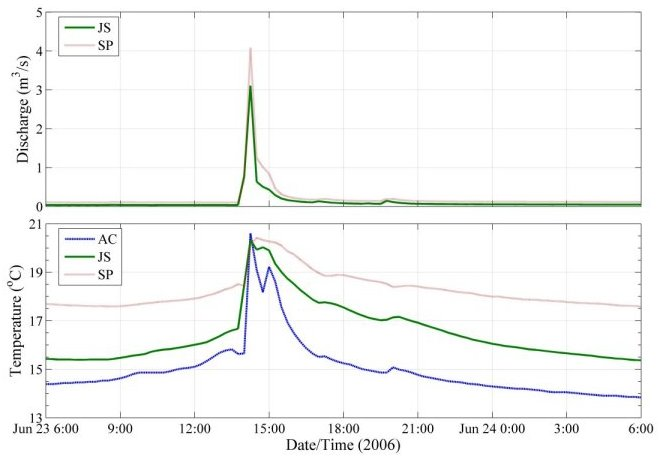
\includegraphics[scale=0.7]{kc_peak.jpg}
\caption[Boone Creek Thermal Charging]{\textbf{\emph{Thermal Charging During Stream Peakflow}} Stream temperature as measured in the highly urbanized Boone Creek during peak stream flow from a storm. Agricultural Center (AC), Jimmy Smith Park (JS) and Steam Plant (SP) indicate measurement positions in a downstream order. The top plot illustrates a spike in steamflow, and the lower plot shows a corresponding spike in stream temperature as a result of some thermally charged point source(s) emptying into the creek. The exact sources for this thermal charging are currently being researched and could include pond overrun or heat from urban surfaces \citep{krautBASE}.\label{kcPeak}}
\end{center}
\end{figure}

These temperature spikes coincide with the onset of sudden afternoon storms that have the capacity for high precipitation rates. This is coupled with the intense heating of urban surfaces that often precedes the afternoon storms. The stormwater channelization from urban surfaces into the surface flow offers virtually no deliberate mechanism for thermal buffering in the current infrastructure regime, and the high precipitation rate ensures that this thermal energy is efficiently evacuated from the surfaces. Additionally, ther thermal charging data presented in Figure (\ref{kcPeak}) supports the hypothesis that shallow retention pond overflow provides a potent point source for themal charging and are not effective best mangement practices (BMP) in their own right \citep{thaxAdd2}. Not only is the retention pond caching solar energy more efficiently than an urban surface during the heating of the day, but it will also receive the potentially hot flash flow from its own catchment.

\subsection{Thermal Remediation Practices}
Current findings and attitudes toward stream restoration agree that the fundamental goal of any restoration effort is to minimize human imposed change on the physical and biological characteristics of a watershed \citep{watersheds,urban}. This does not mean eliminating human activity or impact on the watershed, but instead approaching restoration as a process of mitigating and managing these impacts through well researched methods \citep{rgis}. In the context of thermal remediation, the ideal solutions would involve shade and infiltration. Realistically, dense urban development sheds volumes of stormwater that is obviously proportional to the precipitation, and this is inevitably accumulated, collected and discharged, directly impacting the volume and rate of return in watershed surface and baseflow. The infrastructure pathways that manage this discharge are typically point source outlets in the form of a pipe that releases the stormwater directly into a creek or retention pond. 

Thermally buffering this discharge presents a difficult engineering problem, especially in the situation of upland topography. In upland development real estate is available only at a premium due to the more severe topographical conditions that restrict how and where any sort of development may occur. Sufficiently large retention basins, infiltration zones and even shade are often not practical provisions that accompany dense urban or suburban development in any sort of region, let alone the space-confined upland regions. End-of-pipe and other confined space solutions offer some potential to buffer an initial thermal charge that may accompany a sudden stormwater flush. As shown below, the quantity of aggregate is still significant, and any doctrine for effective thermal buffering would be centered around removing small amounts of heat energy in enumerable locations with small aggregate masses, as opposed to a few large entrenchments with large masses of material. The material does not need to remove all heat energy, but collectively it should exhibit a reasonably large thermal conductivity and specific heat such that the spike of any thermal charge is damped. Optimizing the geometry of aggregate arrangement, type or size of aggregate cobble and maximizing the contact area with discharge flow would be paramount in implementing any sort of solution. 

\subsection{Using Construction Aggregate for Thermal Mitigation}
The focus on construction aggregate is one that stems primarily from a cost to benefit reality, availability and ease of implementation \citep{ballast}. Although it may not be the optimal material, developers have easy access to it and it is affordable. It can readily be installed with minimal effort, although routine maintenance may be required.
 
Construction aggregate is typically available as a regional product. This causes the material of the aggregate to vary considerably which will effect heat capacities, exchange rates and to a lesser degree, flow capacity. Local quarries usually produce a range of cobble sizes, ranging from 3/8'' to 4'' in mean diameter, or more formally measured on site with a series of sieves to rate a particular sample with a fineness modulus. Geometry of the cobbles is always irregular, with some rock types yielding a flatter “chip” type of cobble, which stands to lower the compaction and bulk porosity of the aggregate, at the same time increasing its bulk density. 



%This file will be included in the ThesisMain Document as the experimentation
%section.

%Author: James Kelly
%Last Modified: 10-08-08

%\begin{center}
\section{EXPERIMENTATION}
%\end{center}

\subsection{Stormwater Discharge Simulations}

\subsubsection{Aggregate Samples}
An experiment was devised to measure a thermal exchange between water and a sample of gravel. To measure the exchange in a hydro-dynamic scenario, a so-called stormwater discharge simulator was constructed to flush a body of gravel with heated water at high rates for up to 5 minutes. Temperature sensors measured water temperature and provided time-based temperature data for an analysis of the heat exchange between water and aggregate. In each group of experimental trials, a family of 9 gravel or rock samples was measured (Table \ref{aggsam}), each with a packed volume of 5.60 liters (Appendix A). 

\begin{table}[t!]

\centering                           
\caption[Aggregate Samples]{\textbf{Aggregate Samples}\label{aggsam}} 
\begin{tabular}{l c c c c c c}              
\hline\hline
\\                               
 Material & Diameter & Mass (kg) & ISS (L) & $\frac{n}{kg}$ & Bulk $\rho\;\frac{kg}{L}$
\\[1ex]
\hline 
\\
% Entering 1st row
& $\frac{3}{8}$'' 	& 8.70 	& 2.367	& 1123 	& 1.56\\[1ex]
& $\frac{1}{2}$'' 	& 6.90 	& 2.598	& 201 	& 1.24\\[1ex]
\raisebox{0 ex}{Quartzite}
& $\frac{3}{4}$'' 	& 7.05 	& 2.786	& 80 	& 1.27\\[1ex]
& 5'' 			& 9.00 	& 3.088	& 3 	& 1.62\\[1ex]
\\
\hline
\\
& $\frac{5}{8}$'' 	& 6.35 	& 3.480 & 196 	& 1.14\\[-1ex]
\raisebox{2ex}{Crushed Brick}
& 1'' 			& 5.90 	& 3.556	& 57 	& 1.06\\[1ex]
\\
\hline
\\
& $\frac{5}{8}$'' 	& 7.50 	& 2.608	& 184 	& 1.35\\[-1ex]
\raisebox{2ex}{Marble Cobbles}
& 1'' 			& 7.05 	& 2.675	& 47 	& 1.27\\[1ex]
\\
\hline
\\
Stream Cobble 		& 2'' 	& 10.4 	& 2.556	& 20 & 1.87\\[2ex]
\\
\hline
\\
Siltstone 		& $\frac{1}{2}$'' & 8.9 & 3.191 & 7 & 1.60\\[1ex]
\\
\hline
\\
Steel Balls (1018)	& 1'' 	& 25.0 	& 3.29 	& 15 & 4.50\\[1ex]
\\
\hline
\\
Glass Marbles		& 1''	& 6.50	& 3.21	& 52 & 1.17\\[1ex]
\\
\hline\hline
\end{tabular}
\label{tab:AggSam}
\end{table}

Quartzite and metasiltstone gravel samples were acquired from a local quarry that processes only construction aggregates that are mined on site. These samples include a range of sizes crushed for general construction and asphalt production. Quartzite aggregates are noted for their irregular cobble geometry and relatively high Mohs hardness of 7, which makes it especially suitable for use in non-partitioned arrangements \citeauthor*{ballast}. The other samples were acquired from a local landscaping retailer. Marble garden rocks, though comparably exotic, were selected for their especially high density and heat capacity. The brick sample was simply red, crushed construction brick that was sorted into two general sizes. Round river cobble and red colored medium siltstone were selected for shape and material variation. Finally unplated, mild steel balls (1018 non-annealed alloy) and glass marbles were also tested primarily as theoretically ideal aggregates in one or more thermal parameters.

\subsubsection{Temperature Measurement}
In measuring temperature, HOBO sensors by Onset Solutions were launched and used for each trial, with data being collected from each sensor after every experiment. Each sensor was ultimately modified to provide a 3 second temperature responsivity, as default manufacturer times are well over 5 minutes. The modification involved moving the temperature themistor to the outside of the sensor casing so that it was directly in contact with the fluid, and then re-sealing the unit. 

In Figure (\ref{modSens}) the sensor modification is visible as the protruding temperature element from the end of the sensor body. The semi-conductor that generates the signal for the sensor circuit is encased in a small, black epoxy bulb and this was filed down to further decrease the thermal responsivity with some success. The hole that was drilled in the plastic sensor case was sealed with a a hot/cold temperature cyanoacrylate cement. Before final reassembly, the sensor cavity was filled with a household expanding foam to further protect the sensor circuit from water infiltration. A typical failure mode for this modification was the sensor wires cracking and consequently causing a short circuit. 

\begin{center}
\begin{figure} [h!]
 \centering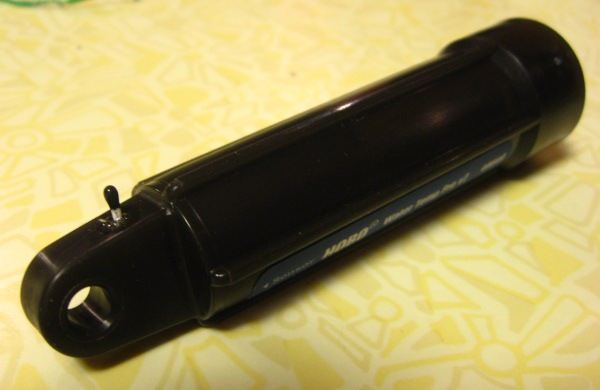
\includegraphics[scale=0.8]{modSensor.jpg}
 \caption[Modified HOBO Sensor]{\textbf{\emph{A modified HOBO sensor}} This shows a HOBO temperature sensor modified to provide better thermal responsivity.\label{modSens}}
\end{figure}
\end{center}

Sensors used in all trials were first matched and calibrated by immersing them in heated fluids and selecting the sensors that only had similar readouts for responsivity and temperature. The modifications induced a greater variance on sensor accuracy, and so this process was implemented to control that. The sensor sampling rate was 1 second, and it was found that the sensors acheived about 50\% true value within that time frame under the most extreme temperature differences. Under the temperature differences found in a single trial, it was observed that such true temperature readings within a sample cycle were much closer, within a degree. 

Measurement error in all data originates with the sensors. There is a temporal error associated not only with just the thermal responsivity but additionally with the synchronization of individual sensors with respect to one another. This synchronization error was found to be up to 1 second in difference and is sourced to the software and personal computer when the sensors are launched. Top and bottom sensors were always carefully ``matched'', in that they measured temperatures very near one another with nearly the same responsivity. A true temperature is not as critical since all fundamental results were interpreted from a temperature difference.

\begin{center}
\begin{figure}[h!]
 \vspace{25mm}
 \centering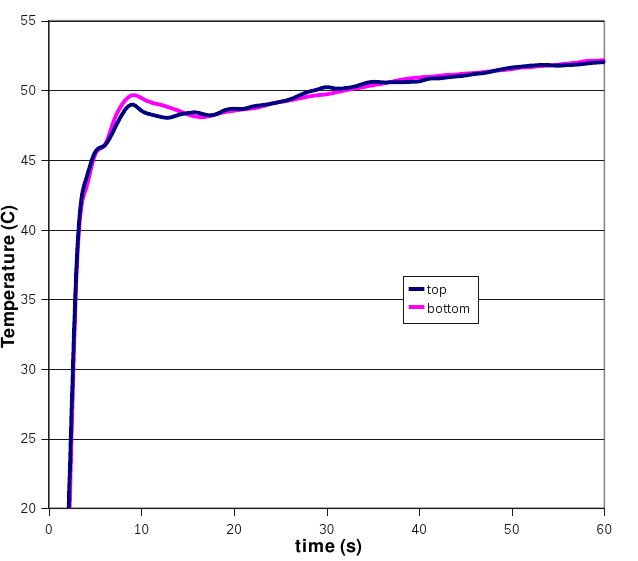
\includegraphics[scale=0.6]{sensorComp1.jpg}
 \caption[Sensor Responsivity]{\textbf{\emph{A comparison of a modifed top and bottom HOBO sensor}} Sensors that had similarly fast responsivity after modification were used to measured the temperature differences across the sample vessel. This match was performed for each trial.\label{sensComp}}
\end{figure}
\end{center}

\begin{landscape}
\begin{center}
\begin{figure}
 \centering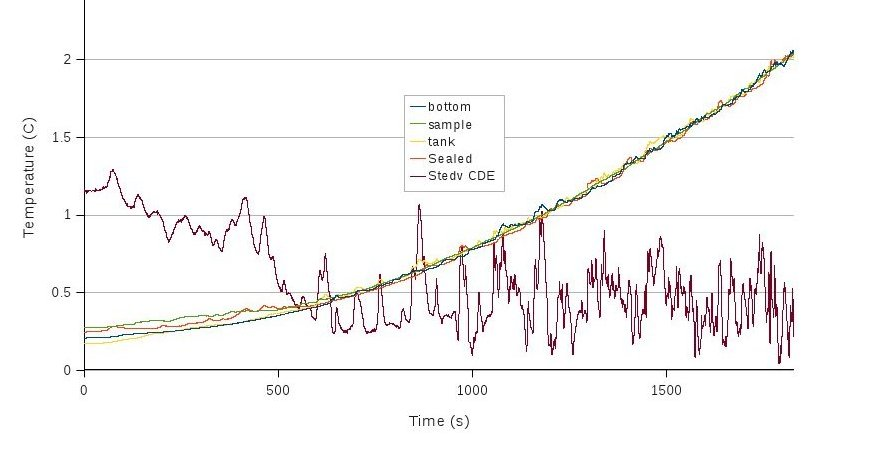
\includegraphics[scale=0.6]{sensorComp2.jpg}
 \caption[Sensor Comparison]{\textbf{\emph{A comparison of modified sensors over a wide temperature range}} This test was performed after a modifcation was implemented to test the long term temperature stability and reliability of modified sensors. In this test, the sensors were immersed in a cold water bath that was slowly heated.\label{sensComp2}}
\end{figure}
\end{center}
\end{landscape}

\subsubsection{Apparatus Construction Basics}
An apparatus was constructed to measure the ability of an aggregate sample to thermally sink a continuous flow of heated water. The apparatus consisted of a main circuit through which heated water was continuously circulated from a reservoir and afterwards discharged. The vessel that contained the aggregate sample was oriented vertically, with hot water introduced at the top of the vessel. Using HOBO sensors, flow temperature was measured before the water entered the sample vessel, and after. A flow sensor measured the flow rate shortly after the sample vessel. Figure (\ref{discharger}) is a schematic illustration of the apparatus, its flow design and the sensor loctions. Photographs of the operational apparatus are shown in Figures (\ref{dischargerPhoto}) and (\ref{vesselPhoto}). 

\begin{center}
\begin{figure}
\noindent
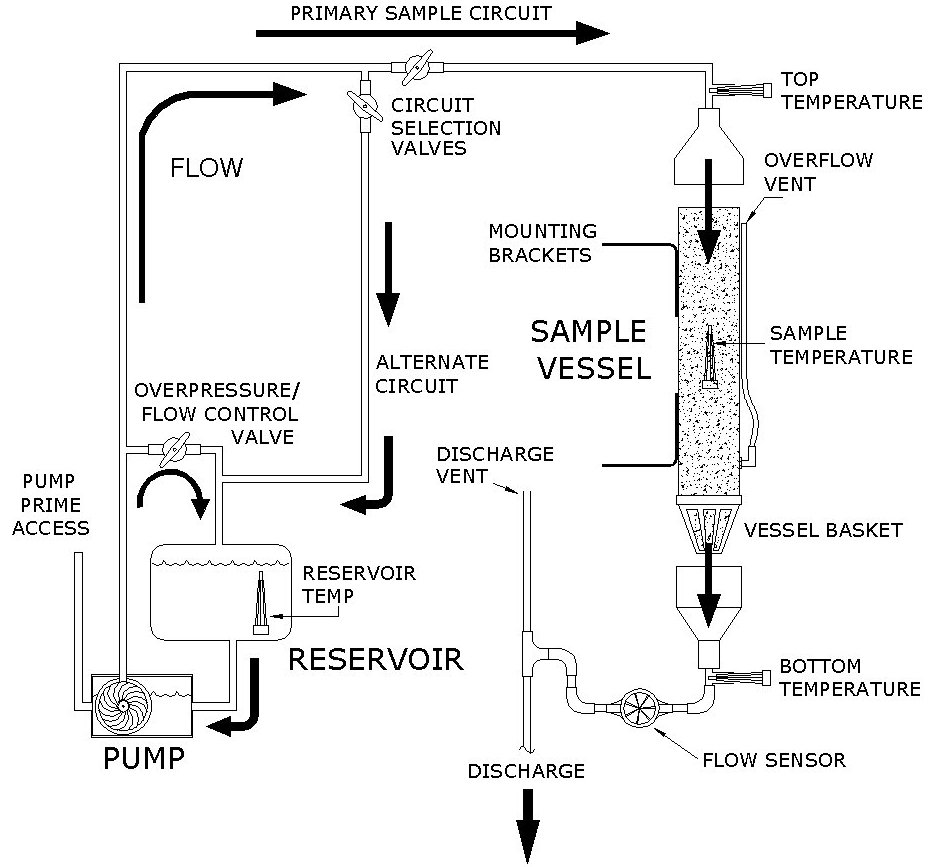
\includegraphics[scale=0.5]{DISCHARGER.jpg}
\caption[Stormwater Discharge Simulator Schematic]{\textbf{\emph{Schematic Diagram of the Stormwater Discharge Simulator}}\label{discharger}}
\end{figure}

\begin{figure}
 \centering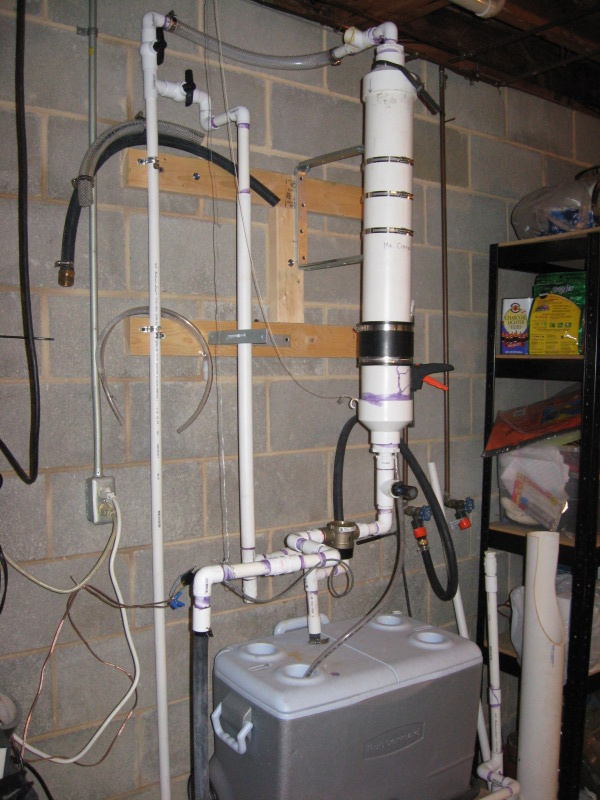
\includegraphics[scale=1.25]{dischargerPhoto.jpg}
 \caption[Stormwater Discharge Simulator]{\textbf{\emph{The assembled stormwater discharge simulation apparatus.}}\label{dischargerPhoto}}
\end{figure}
\end{center}

\begin{figure}
\centering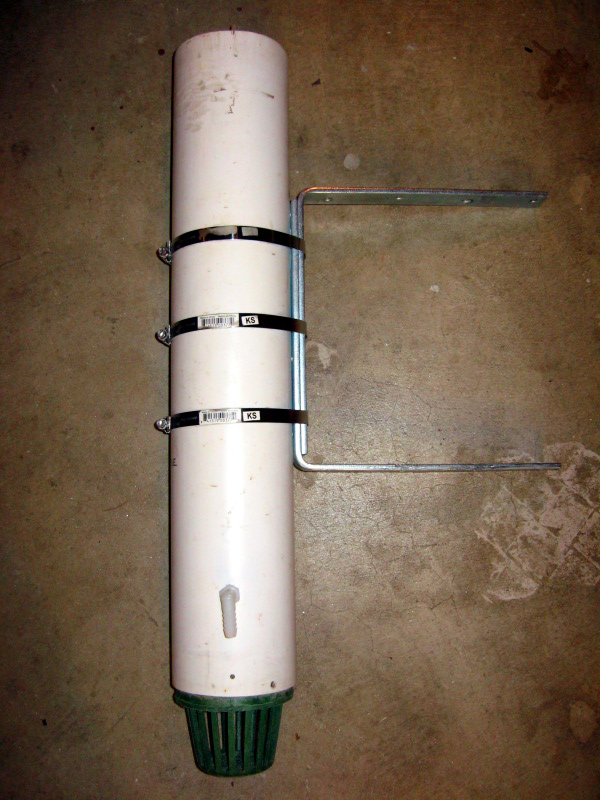
\includegraphics[scale=1.25]{vesselPhoto.jpg}
\caption[Sample Vessel]{\textbf{\emph{Sample vessel is shown seperated from the main circuit.}}\label{vesselPhoto}}
\end{figure}

\subsubsection{Apparatus Operation}
A sample or aggregate material was dumped into the vessel, which was removed from the main circuit. Figure (\ref{isovessel}) illustrates a cross section of the sample vessel, the sample aggregate and the vessel dimensions. The sample was checked for correct packing and the vessel was installed into the main circuit to complete the assembly of the apparatus. The reservoir was filled with 40 liters of water typically heated to 45-50 $^{o}$C. Run-time specifics are tabulated in Table (\ref{simNom}).

\begin{figure}[h!]
\centering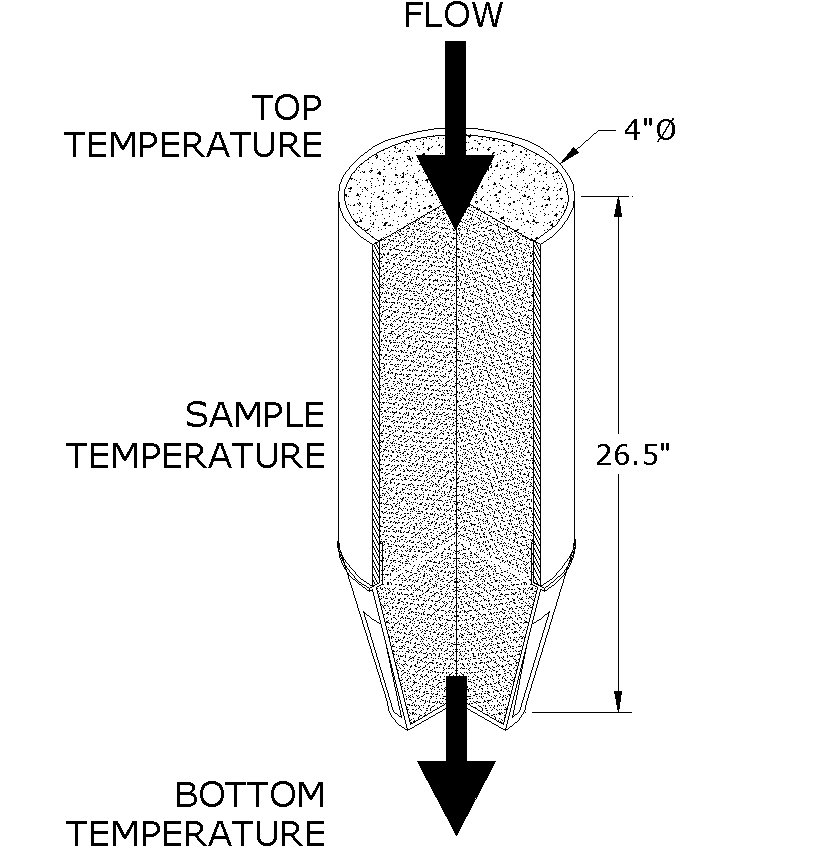
\includegraphics[scale=.35]{isoVessel.jpg}
\caption[Sample Vessel Cross Section]{\textbf{\emph{Sample vessel dimensions and cutaway with temperature probe locations.}} (The figure is not drawn to scale.)\label{isovessel}}
\end{figure}

An electric centrifigal pump was used to circulate water from the reservoir up to the top of the sample vessel. The pumping rate was adjustable with a gate valve that returned a certain fraction of the flow to the pump prime. The sample vessel was 4'' in diameter and 26.5'' in length, cut from a length of schedule 40 PVC. A drainage basket was fitted into the end to restrain the sample, yet afford minimal flow obstruction. The vessel performed as a gravitationally charged fluid coupling, through which water freely flowed through the interstitial space of the aggregate. Because gravity drives the flow, the type of aggregate not the pumping rate, was the dominant control of flow in the vessel. It should be noted that the maximum flow rate produced by the pump was accomodated by all aggregate samples. This was verified by the use of a clear overflow vent tube installed in the side of the sample vessel. If the net inflow were to exceed the effluent, the accumulation of fluid relative to the vessel height would appear in the clear vent tube, and this was never observed during a trial in which data was collected.

A second flow circuit was used to circulate water before the trial was to begin. This second circuit paralleled the primary sample circuit, except branching off just prior to the top temperature sensor and bypassing the sample vessel, returning all water to the reservoir. This circuit was used for 2-3 minutes prior to flushing the sample, and then disabled with a gate valve once the main circuit was opened. This recirculatory circuit was used to flush out cold pump prime water and to heat the circuit piping and brass pump head prior to collecting data. This warm-up helped to normalize the energy flow into the sample vessel and provided an initial thermal charge with a temperature closer to the actual reservoir temperature. The reservoir temperature dropped nominally when turning on this circuit. 

\begin{table}[ht!]
\caption[Experiment Nomenclature]{\textbf{Experiment Nomenclature}\label{simNom}}
\centering
\begin{tabular}{r l l}
Parameter & Abbreviation & Units\\
\hline
\\[-.5ex]
Fluid (Water)					&	$W$\\[3mm]

Aggregate Material or Sample			& 	$R$\\[3mm]

Energy						&	$Q$			& $J$\\[3mm]

Net Energy Exchange [Source -- Sink]		&	$Q_{net}[W-R]$		& $J$\\[3mm]

Time Step Energy Exchange [Source -- Sink]	&	$Q(t)[W-R]$		& $J$\\[3mm]

Volumetric Heat Capacity of Fluid (Water)	&	$Cv_{W}$		& $\dfrac{J}{L*K}$\\[3mm]

Bulk Specific Heat of Aggregate			&	$c_{R}$			& $\dfrac{kJ}{kg*K}$\\[3mm]

Bulk Heat Capacity of Aggregate			&	$C_{R}$			& $\dfrac{kJ}{K}$\\[3mm]

Vessel Residency Time 				&	$t_{V}$			& $s$\\[3mm]

Aggregate Bulk Specific Gravity			&	$\rho_{R}$		&\\[3mm]

Aggregate Bulk Thermal Conductivity		&	$\kappa_{R}$		& $\dfrac{W}{m*K}$\\[3mm]

Aggregate Bulk Thermal Diffusivity		&	$\alpha_{R}$		& $\dfrac{m^{2}}{s}$\\[3mm]

Aggregate Mass					&	$m_{R}$			& kg\\[3mm]

Average Top Sensor Temperature 			&	$T[TOP]$		& $^{o}C$\\[3mm]

Time Stepped Bottom Sensor Temperature 		&	$T(t)[BOTTOM]$		& $^{o}C$\\[3mm]	

Fluid Flow Rate (L/s)				&	$\nu_{W}$		& $\dfrac{L}{s}$\\[3mm]

Top - Bottom Temperature Difference 		&	$\Delta T[TB]$		& $^{o}C$\\[3mm]

Time Stepped $\Delta T[TB]$ 			&	$\Delta T(t)[TB]$	& $^{o}C$\\[3mm]

Ambient Temperature				&	$T[AMBIENT]$		& $^{o}C$\\[3mm]

\hline
\end{tabular}
\end{table} 

\subsection{Flow Sensor Data Acquisition and Interface}
A rotary vane type flow sensor with a 3/4'' diameter aperature was placed inline with the outgoing flow. This particular sensor generated a digital 5V output signal that coincided with the flow rate. To generate this signal, the sensor itself was driven by 5V DC, rated at 40 mA. This digital signal was read by a single data input (address = 3F8h) on a personal computer parallel port. The port was sampled at 1kHz, which restricted the maximum measurable input signal to about 330 Hz. This was found to coincide with a flow rate of about 3 L/s, well below the apparatus' pump capacity.

On the personal computer, a data acquisition (DAQ) front panel (Figure \ref{frontpanel}) was coded in Visual Basic (6.0) to sample the parallel port and to convert the signal to a real-valued flow rate. The front panel was first calibrated using gravitationally driven flows of a known volume at various flow rates. An order 3 polynomial calibration curve was then formulated from this data and used by the front panel to determine flow rate. Errors encountered in the calibration of the flow sensor were two orders of magnitude less than the manufacturer's specificed measurement error of $\pm10\%$. 

\begin{figure}[ht!]
 \centering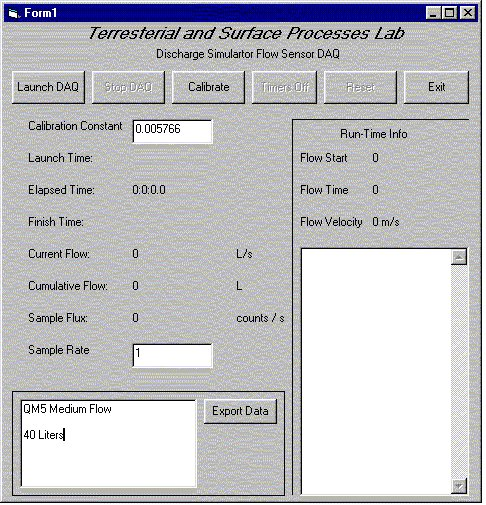
\includegraphics[scale=.65]{frontpanel.jpg}
 \caption[Front Panel Screen]{\textbf{\emph{Front Panel of the Data Acquisition (DAQ) interface}} This Visual Basic front panel was designed to time only active flow (non-zero) and to export the data batch as a tab-delimited ASCII text file. A high precision timer (RSTimer) was used to sample data from the parallel port at 1kHz, and to create flow rate data with one second resolution. Before each trial, this timer was synchronized with the temperature sensors.\label{frontpanel}}
\end{figure}

\begin{figure}[ht!]
 \centering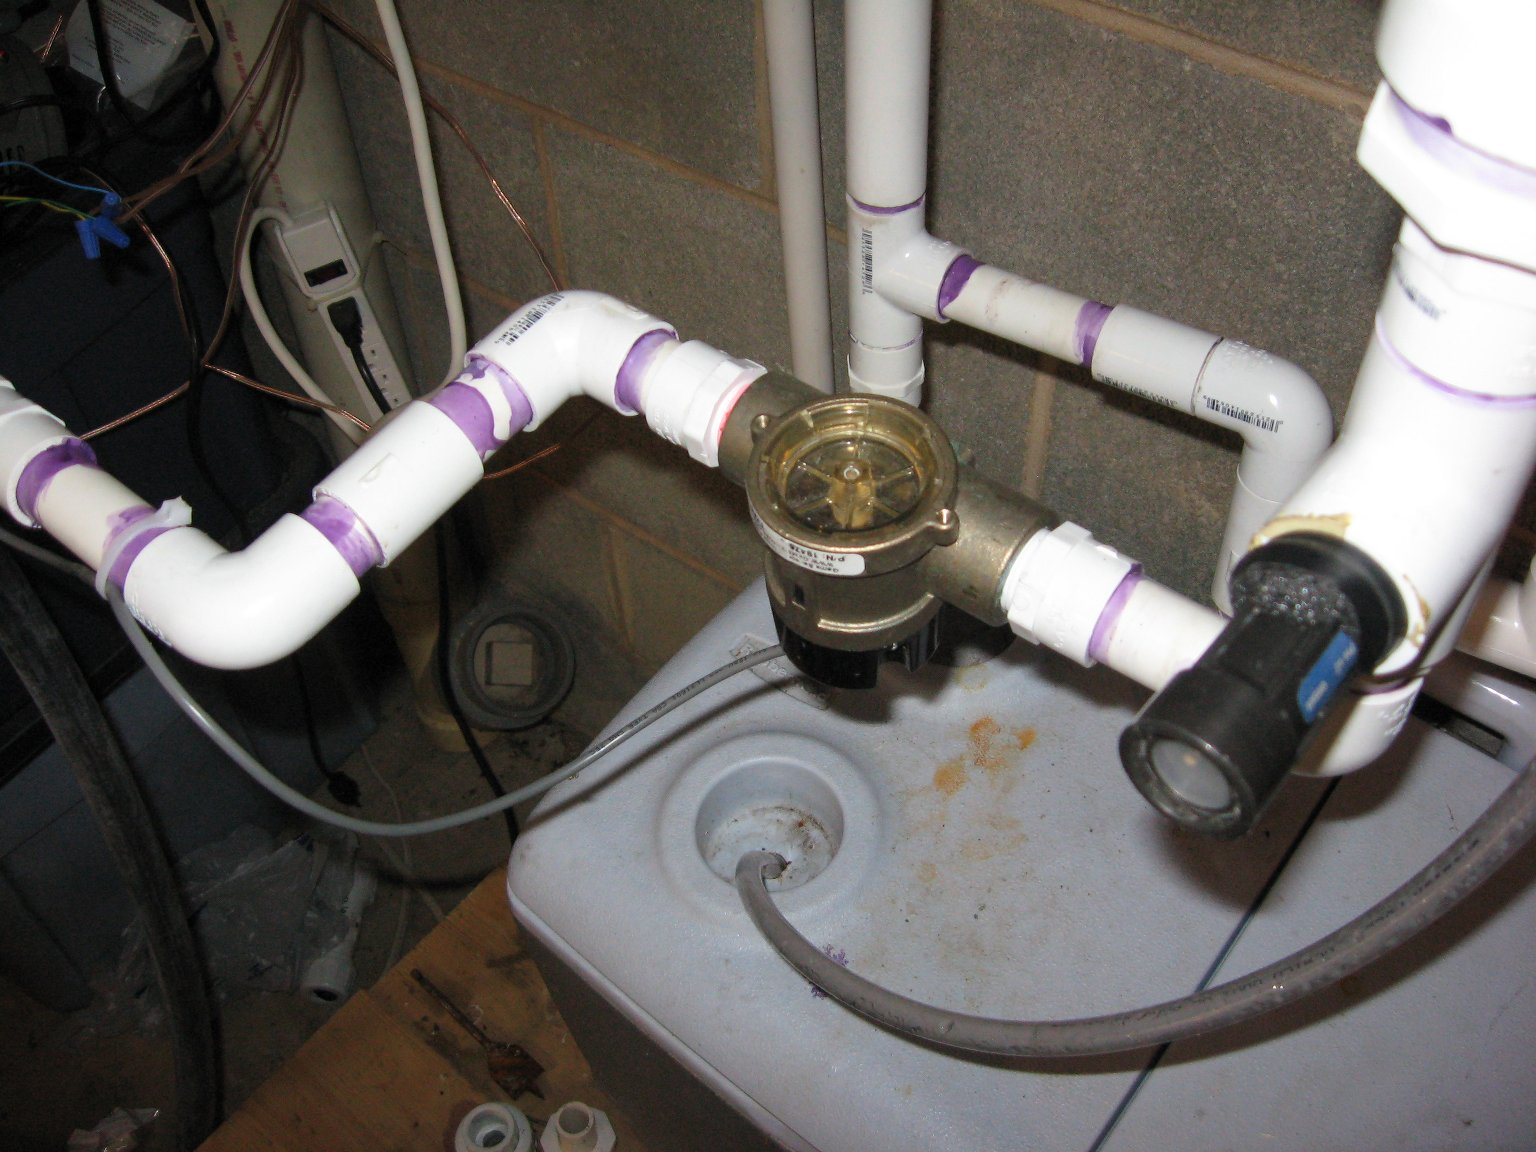
\includegraphics[scale=.25]{flowsens.jpg}
 \caption[Flow Sensor]{\textbf{\emph{Photograph of the Operational Flow Sensor}}\label{flowsenser} Shown is the rotary vane type flow sensor that was interfaced to the Visual Basic Front Panel. Visible is the bend in the plumbing following the sensor that served to create some backpressure to limit the air bubble ingestion of the rotary vane chamber.}
\end{figure}
\pagebreak
\subsubsection*{Run-Time Specifics}

When conducting a trial, the following procedure was followed to carry out a single flow experiment:

\begin{itemize}
 \item The two personal computers that manage data collection are time syncronized via a network connection. This is typically  done only once every hour. 
\pagebreak
 \item The temperature sensors are first launched and installed in their respective positions around the circuit.
	\subitem Reservoir Sensor (Tank)
        \subitem Internal Vessel Sensor (Sample)
	\subitem Sensor above the vessel (Top)
        \subitem Sensor below the vessel (Bottom)
\pagebreak
 \item Each sensor is configured to begin data recording at a common time to allow for easy time syncing of data. The sensors are ultimately verified that they are active before following through with the trial.
 \item The reservoir tank is filled with 40 liters of hot water at $\sim48^{o}\,C$.
 \item The vessel is verified by touch that it has cooled if the current run trails another. No less than 10 minutes were allowed between trials. The vessel is then filled with an aggregate sample. Aggregate samples were unchanged for all trials. Only dry, room temperature aggregates were used for trials.
 \item The vessel is connected to the circuit. Precautions were taken to ensure no circuit leakage, and no trials exhibited any measurable fluid loss.
 \item The secondary circuit is opened and the pump is switched on, allowing a warming of the inflow piping. 
 \item The flow sensor is turned on and inspected for debris or obstructions. The DAQ front panel for the flow sensor is activated and records a time stamp.
 \item With respect to the DAQ time stamp, the secondary circuit is turned off after no less than 2 minutes. By design, once the secondary circuit is deactivated, water is then directed into the main sample circuit. 
 \item The flow sensor DAQ is activated once the flow sensor receives flow. The interface then begins recording flow data every second.
 \item The trial will last anywhere from 40-300 seconds, dependent on flow rate. A restrictor valve at the pump head can be manipulated to redirect a fraction of flow back into the pump prime. This was used only to achieve low, medium and high flow rate trials and was not adjusted during a data collecting trial.
 \item Once the pump prime has run dry and flow has ceased, the main circuit is closed. Flow sensor data is retrieved from the front panel and the DAQ is shut down.
 \item The sensors are removed from the circuit and the vessel is disconnected.
 \item The sample is emptied to dry in a seive and a small fan is placed in the vessel to cool and dry it for the next trial.
 \item Data is removed from the temperature sensors and they are shut off. Figure \ref{rawTemps} illustrates a sample output of raw data.
\end{itemize}
\begin{landscape}
\begin{figure}
\begin{center}
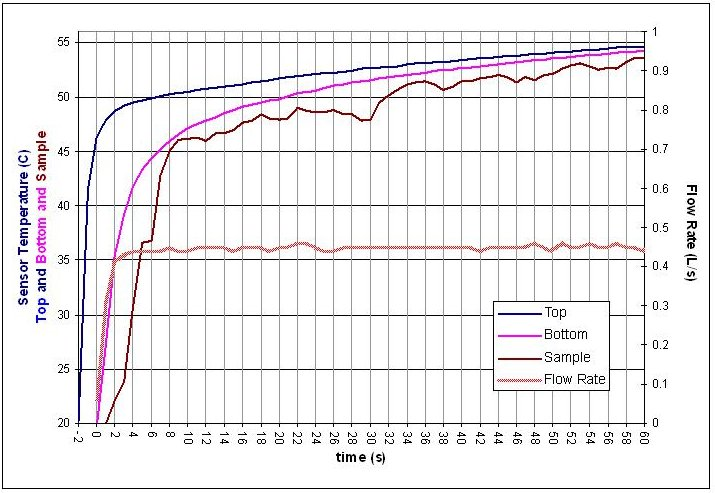
\includegraphics[scale=.65]{rawTemps.JPG}
\caption[Raw Temperature Plot]{\textbf{\emph{Raw Temperature Data from a Single Trial}} Temperature data sources depicted are top, bottom, and sample sensors with a flow rate plot on the right axis.\label{rawTemps}}
\end{center}
\end{figure}
\end{landscape}

\begin{table}[ht!]
\caption[Simulation Run-Time Statistics]{\textbf{Simulation Run Time Statistics}\label{runTime}}
\centering
\begin{tabular}{r l}
\hline
\hline
\\[-.5ex]
Data Time Resolution    & 1 second (all sensors)\\
\\
Reservoir Capacity	& $\lessapprox 40\;L$\\
\\
Reservoir Temperature 	& $43-51^{o}\;C$\\
\\
Fluid 			& Heated Tap Water\\
\\
Flow Rates		& 23 (Low), 41 (Med), 52 (High) $\frac{L}{s}$\\
\\
Flow Sensor		& $\frac{3}{4}''$ Digital Rotary Vane $\pm10\%$\\
\\
Flow Sensor Capacity	& 0.15 - 2.45 L/s\\
\\
Typical Flow Times (sec)& 190 (Low), 95 (Med), 65 (High)\\
\\
Sample Circuit Length	& 6.70 meters $\pm0.3\;m$\\
\\
Circuit Piping		& SCH 20 PVC $\frac{3}{4}''\varnothing$\\
\\
Vessel Dimensions	& 4'' x 27'' (10 x 69 cm)\\
\\
Vessel Volume		& 5.83 L\\
\\
Vessel Material		& SCH 40 PVC 4''$\varnothing$\\
\\
Typical Sample Mass	& 4.5-4.9 kg\\
\\
Pump Specification	& $\frac{1}{2}$ hp electric centrifugal @ $2000\;\frac{L}{hr}$\\
\\
\hline
\end{tabular}
\end{table} 

\subsubsection*{Apparatus Error and Calibration}
It was found that all samples were thermally exhausted within the amount of time 40 litres of water was flushed, regardless of rate, and this was the usual quantity circulated for a single trial. Background loss trials were performed demonstrating energy losses inside the vessel did not exceed the signal noise of the temperature sensors, and such this noise was not subtracted or otherwise considered in data analysis.

The flow sensor was calibrated using various known gravitationally driven flow rates. The circuit was plumbed to afford a continuous backpressure on the sensor to limit turbulent flow and air bubble contamination in the rotary vane cavity. Additionally, the effluent downspout was top vented so that the outflow would not siphon or draw additional flow through the sensor. Despite these provisions, the flow sensor was observed to ingest significant air and endure periodic turbulent flow, based on the driving flow rate. Further more, the rotary vane has a manufacturer tolerance of $\pm$10\%. While some of the turbulence and flow error has been absorbed into the interface calibration, the meter still demonstrated some error as a function of flow rate. For each trial, the reservoir was carfully filled to 40 litres (unless otherwise specified) and flow losses were neglected. A linear flow correction ratio was then computed for each data set.

\[flow\:correction\:ratio\;=\frac{measured\;cumulative\;flow}{measured\;reservoir\;volume}\]

In normalizing temperature differences and in an attempt to generate ideal data sets, the alternate warming circuit was used to achieve nominal differences between the top and reservoir temperatures at run time. Temperature differences between the top and reservoir sensors were never exactly $0^o\;C$ and varied exponentially as a function of time during the actual trial. This difference will partially be absorbed in the data analysis by only considering temperature differences across the vessel, but it will remain a known source of noise and curve distortion. 

The HOBO sensors were always calibrated and paired for use across the the vessel. However, no two sensors were measured to be exact, especially with respect to responsivity and accuracy. The sensors were not manufactured for fast responsivity and the aforementioned modifications increased the variability of each sensor, in exchange for dramatically faster responsivity. Variations in sensor readings were most notably manifested in offset equilibria, or a failure for the vessel temperature difference to reach $0^o\;C$, even when the aggregate was clearly thermally saturated. 

Because the temperature sensors were recording temperature continuously and were not triggered, the temperature data that was recorded across the sample vessel was unsynchronized with respect to the flow. The bottom temperature sensor was effectively reading the water temperature up to 6 seconds after the top sensor due to the vessel residency time of the flow. 

\[Vessel\:Residency\:Time\;=\;\frac{Vessel\:Length}{Flow\:Velocity}\]

\noindent Where the flow velocity is actually an involved empirical function of gravity, aggregate fineness, pump flow rate and aggregate packing ratio. This is discussed in the theory section. 

Sample, top and bottom temperature derivatives were plotted and time shifted such that the rise in temperature due to flow for each sensor was aligned in the time domain (refer to Data Analysis section). The time shift also offers an approximate determination for vessel residency time and vessel flow velocity. There is significant error in this detmination since both sensors cumulatively can produce an error of $\pm2$ seconds due to sampling syncopation and instrument timing variations. However, it does provide a useful baseline to compare flow differences between aggregates. 

Inflow was observed to be sufficiently turbulent such that there was no preferential flow into or about the sample. Additionally, all cobbles were noted to be equally well heated by touch upon emptying the vessel with no dry or cold ``spots''. Trials were run exclusively in ambient temperatures of $19-22^{o}\;C$. It has been hypothesized with some supporting data that the largest sources of error in the measurement of temperature was the sensors themselves and the variant reservoir temperatures.
%\doublespacing

\begin{center}
\section{Data Analysis}
\end{center}

Temperature data read from the HOBO sensors was aligned and cropped with respect to the actual trial. This prepared data included 5 sensor data sets: bottom, sample, tank and top temperatures, and flow data. Flow data was available in liters / second directly from the front panel output program. The flow data was used to locate the time frame in which the trial occured, and the temperature data was then cropped accordingly, timestamped and archived as a final trial dataset. This dataset was inserted into a spreadsheet template that performed the following analyses and calculations.

\subsection{Time Synchronization of Temperature Data}
Temperature data collected from the HOBO sensors was first synchronized in the time domain to account for vessel transience (Figure \ref{timeSync}). This amounted to a specific residency time that was primarily dependent upon the aggregate cobble size. The bottom temperature second derivative was numerically aligned with the top temperature second derivative, with the assumption that some thermal energy would be promptly measured by the bottom sensor despite thermal sinking effects. In Figure \ref{timeSync} the left plot images the first derivative of top, sample and bottom temperatures for a flow of 0.4 liters / second using a sample of glass balls (G1). The right plot is the time synchronized re-plot that results in the temperature data being temporally aligned. 

\begin{landscape}
\begin{figure}
\begin{center}
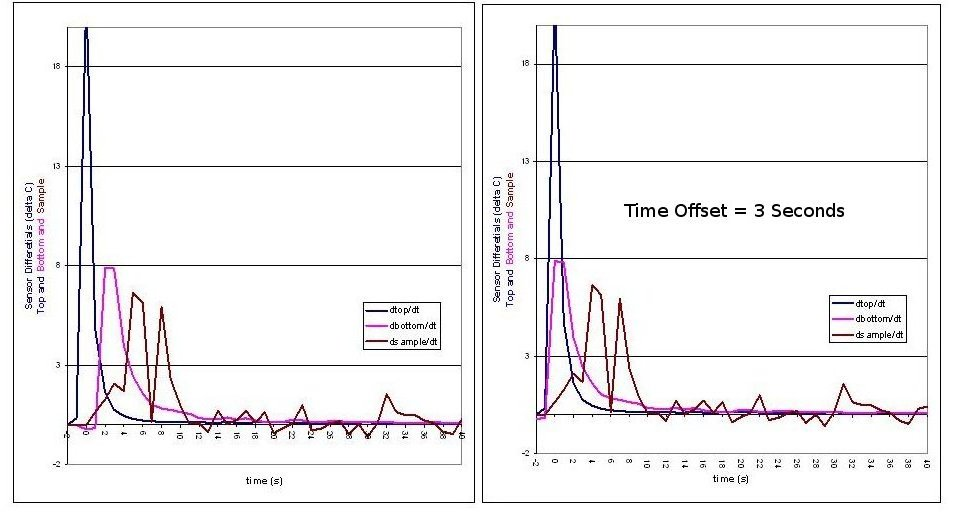
\includegraphics[scale=.6]{sideBYsideSync.jpg}
\caption[Vessel Temperature Differences]{\textbf{\emph{Non-synchronized and Synchronized Vessel Differential Temperature Data}}  The figure on the left shows first-derivative temperature data that is not time synchronized. The figure on the right shows first-derivative temperature data that has a bottom temperature shifted -3 seconds to be aligned with the top temperature readings. By aligning the rate of change of the temperature sensors, flow percolation time is removed from energy transfer anlyses.\label{timeSync}}
\end{center}
\end{figure}
\end{landscape}

\begin{landscape}
\begin{figure}
\begin{center}
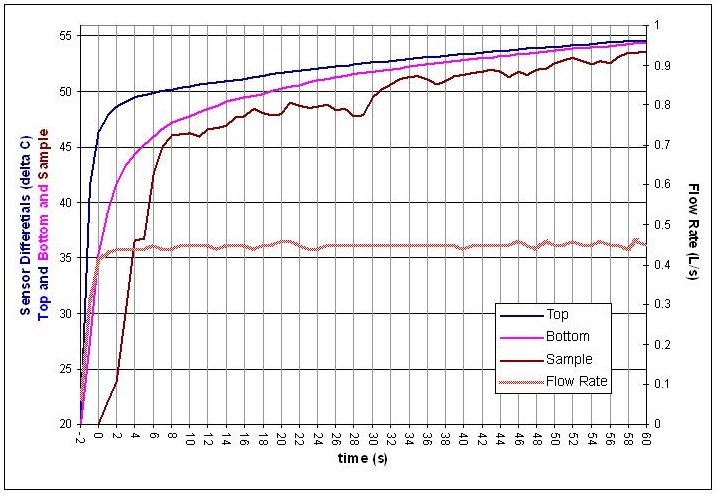
\includegraphics[scale=0.6]{timeSyncTemp.JPG}
\caption[Synchronized Temperature Data]{\textbf{\emph{Synchronized Temperature Data}}Top and Bottom temperature data is aligned in the time domain.\label{syncTemp}}
\end{center}
\end{figure}
\end{landscape}

Note that despite temporal alignment, Figure (\ref{timeSync}) illustrates a sample temperature that remains offset due to intermittent flow contact. The inflow fluid rate is insufficient to completely saturate the volume afforded by the interstitial space, and there is consequently a fractional contact between the fluid and cobbles. The noise of the sample temperature data affirms this. To intuitively align the sample data in this example, a time offset greater than the bottom offset is needed, which is physically meaningless. All temperatures and temperature differences used in analysis and theory sections has been temporally aligned with respect to vessel residency time. 

\subsection{Vessel Temperature Differential}
The synchronized temperature data was subtracted and plotted in Figure (\ref{tempDiff}).  
\[T(t)[TB]=T(t)[TOP]-T(t)[BOTTOM]\]
This quantity represents the time stepped, synchronized temperature difference across the vessel, identifying the driving potential for energy transfer. The time where this temperature difference fell below 0.12 $^{o}$C is defined as the positive thermal sink time and is denoted as $t_{+Q}$. This point identifies where the heat effectively ceases to flow from the fluid to the rock and is the key marker in performing additional analyses. The threshold of $t_{+Q}$ is determined from average sensor noise acquired during sensor calibrations and responsivity.
\pagebreak
\subsection{Cumulative Energy Transfer}
Once the data are aligned in the time domain, or synchronized, each time step is used to compute a top-bottom temperature difference. This difference is plotted over the time domain in Figure (\ref{tempDiff}). This curve is then numerically integrated according to the following theory.

\noindent The cumulative energy exchanged between the flow and the aggregate can be expressed as
\[\int \varphi T(t)dt=Q(t)[WR]\]
Where
\[\varphi = \nu_{W}Cv_{W}\]
Numerically Integrating from $t=0$ to $t_{+Q}$
\begin{equation}\label{NSCF}
\sum_{ti}^{t_{+Q}}\left[\left(\varphi\right)T(t)[TB]dt\right]=Q_{net}[WR]
\end{equation}

This method produces an integral function that can be interpreted as the cumulative energy transfer of the flow, or total heat loss from the water. The curve itself describes both the rate of energy transfer and the total quantity of thermal energy cached by the sample, and it provides the basis for further analysis of the samples' thermal sink characterization.

\begin{landscape}
\begin{figure}
\begin{center}
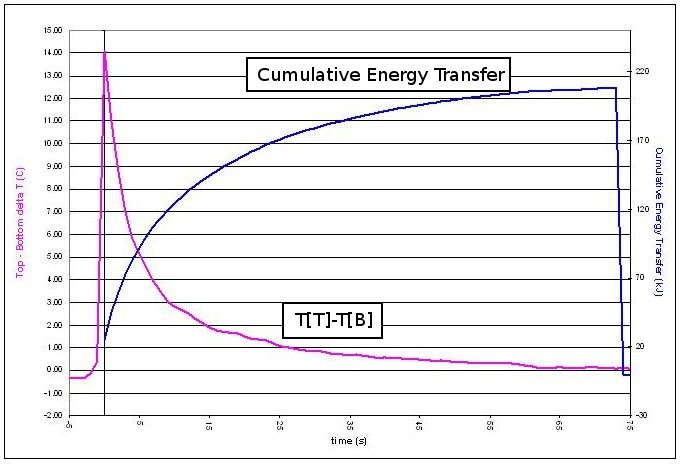
\includegraphics[scale=.65]{tempDiff.JPG}
\caption[Temperature Difference and CET Plot]{$T[T]-T[B]$ plot illustrates the temperature differences between the top and the bottom of the sample vessel along with the total thermal energy exchanged between the fluid flow and the sample - cumulative energy transfer. This example was performed with glass marbles (G1) at a flow rate of 0.40 L/s.\label{tempDiff}}
\end{center}
\end{figure}
\end{landscape}

\subsection{Normalization of the Cumulative Energy Transfer Function}
In comparisons of cumulative energy transfer (CET) functions, between different aggregates or even between different trials of the same aggregate, it is necessary to scale the data for the variances in reservoir temperature. 

\noindent From the First Law of Thermodynamics, and neglecting systemic losses,
\[-Q(t)[W]=Q(t)[R]\]
and the definition of heat transfer at constant pressure,
\[Q=mc\Delta T\]
\begin{equation}\label{specheat}
\varphi\Delta T(t)[TB]=m_{R}c_{R}\Delta T(t)[R] 
\end{equation}
The total heat lost by the fluid flow can be expressed in a time-stepped form as
\begin{equation}\label{Qt}
Q(t)[W]=[\varphi t]\Delta T(t)[TB]
\end{equation}
or as a net quantity over the entire positive thermal sink time, $t_{+Q}$
\begin{equation}\label{Qnet}
Q_{net}[W]=\varphi t\;\sum_{t=0}^{t_{+Q}}\Delta T(t)[TB]
\end{equation}
From (\ref{Qnet}) and (\ref{specheat}) the specific heat of the aggregate is computed as
\begin{equation}\label{cr}
c_{R}\;=\;\dfrac{t_{+Q}Cv_{W}\sum\Delta T(t)[TB]}{m_{R}\left(T[TOP]-T[AMBIENT]\right)}
\end{equation}
Where $T[AMBIENT]$ is used as the minimal thermal potential available at run-time and is acquired from all four temperature sensors while they are installed in the apparatus before the trial begins.

The average rock temperature as a function of time, T(t)[R] is then inferred from the time-stepped equivalent of this expression by way of the first law of thermodynamics.
\begin{equation}\label{crt}
c_{R}\;=\;\frac{t_{+Q}Cv_{W}\Delta T(t)[TB]}{m_{R}\left(T[TOP]-T[AMBIENT]\right)}
\end{equation}
and using (\ref{specheat}) with (\ref{cr})
\begin{equation}\label{rt}
T(t)[R]\;=\;\dfrac{-\Delta T(t)[TB]}{\sum\Delta T(t)[TB]}\left(2T[TOP]-T[AMBIENT]\right)
\end{equation}

Equation (\ref{rt}) is a theoretical approximation that figures aggregate temperature with respect to time is purely a function of energy exchange and heat capacties. While this is an accurate assumption, the theory section elaborates on some of the more sophisticated underpinnings that define the aggregate's thermal gradient.

A differential equation solution formulating the rate of energy exchange between the fluid and the aggregate is used as a first order approximation model of the temperature change of the aggregate. Ultimately, this will allow the data to be scaled to match other cumulative energy transfer plots for direct graphical comparison. 
\begin{equation}
\frac{T(t)[WR]}{dt}=-\sigma T(t)[WR]
\end{equation}
Where $\sigma$ is a time constant or rate of heat loss per unit time. This equation has a solution that is realized as Newton's Law of Cooling except with a reversed heat flow. The driving mechanism of thermal potential remains the same, except heat is flowing from a reservoir to a sink. 
\begin{equation}\label{dffsoln}
T(t)[WR] = T_{o}e^{-\sigma t}
\end{equation}
Where $T_{o}=T[TOP]-T[AMBIENT]$ as an initial condition of the differential solution.
This function that is used to scale is actually an algebraically simplified ratio of the form
\begin{equation}\label{simDiffEq}
\dfrac{\Delta T(t)[TB]}{\sum\Delta T(t)[TB]}\;=\;e^{-\sigma t}
\end{equation}
Where sigma represents a time constant comprised of intrinsic and environmental parameters and is elaborated on in the theory section of this document. Numerically, the left hand side of (\ref{simDiffEq}) is used to plot and compute time stepped cumulative energy transfer values.

In scaling a cumulative energy transfer function for a particular trial, the left hand side of \ref{simDiffEq} is plotted against time (Figure \ref{corrPlot}). This curve exactly mimics the shape of the cumulative energy transfer plot; however it is dimensionless and serves as a good visual comparison with other trials. 

\begin{figure}[h!]
\begin{center}
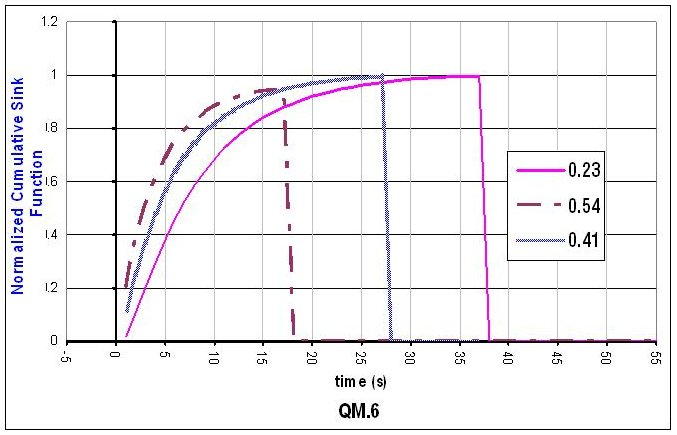
\includegraphics[scale=.6]{correctedPlot.jpg}
\caption[Normalized CET Plot]{\textbf{\emph{A Normalized Cumulative Energy Transfer Function}} An integrated or cumulative energy transfer function is shown after the scaling method summarized in Equations (\ref{rt}) and (\ref{simDiffEq}). A comparison between different sink parameters of the same aggregate can easily be interpreted from this plot.\label{corrPlot}}
\end{center}
\end{figure}

While it is tangent to the process of normalizing the cumulative energy transfer functions, it is worthwhile to point out a relationship that is derived from this formulation:
\begin{equation}\label{tt}
\frac{\Delta T(t)[WR]}{T_{o}}\;=\;\frac{\Delta T(t)[WR]}{\sum\Delta T(t)[TB]}
\end{equation}
It is important to point out a pivotal assumption in this relationship: $T(t)[WR]=T(t)[TB]$. This is of course true at $t_{+Q}$ but only true \emph{on average} over the length of the vessel between $t=0$ and $t_{+Q}$. In these calculations then, it is important to note that the aggregate as a whole is blackboxed and treated as a bulk thermal sink. In the theory section the underlying mechanics of heat exchange inside the vessel will be discussed.

\subsection{Thermal Power Calculations}
Thermal power into and out of the aggregate vessel is computed to provide a numerical conceptualization of thermal sink characteristics and intermediate calculations for other thermal parameters. The time-stepped thermal power of the water column as it flows into the vessel is computed relative to the ambient temperature.

\begin{equation}\label{pin}
P[TOP]=\left(T[TOP]-T[AMBIENT]\right)\left(\varphi (t)\right)
\end{equation}

\noindent with each time step at 1 second to dimensionally arrive at J/s.

\noindent The power out of the vessel is computed in a similar way.
\begin{equation}\label{pout}
P[BOTTOM]=\left(T[TOP]-T[BOTTOM]\right)\left(\varphi (t)\right)
\end{equation}

\noindent The thermal sink power is the difference of the power of the flow in and the power of the flow out and is on the order of several kW. 
\begin{equation}\label{tsp}
P[R]=P[TOP]-P[BOTTOM]
\end{equation}

These values are useful as thermal discharge regulations are defined in terms of net energy \citep{EPA}. In recommending aggregates for thermal sink applications, a particular cobble size and material can be selected based on similar power calculations to meet specific thermal TMDLs \citep{urban}.

\subsection{Bulk $\kappa$ and $\alpha$ Calculation}
Thermal conductivity is approximated under the assumption that heat transfer inside an individual cobble is a linear transfer rate only for a comparatively short period of time while subjected to thermal duress. This assumption is compounded by significant measurement error, and the actual thermal diffusivities are computed only as a means of comparison and experiment, and not as an actual measurement of the aggregate. It should be noted that a theoretical approach was attempted using the heat equation with a floating boundary condition to represent the bottom temperature. It was determined that such a solution was unnecessarily complex, especially when results were so effectively described by the solutions mentioned in the theory section. A heat equation solution is still possible, and may be sufficiently simplified under certain conditions to be useful in providing a reliable thermal conductivity.

For each aggregate trial, the time step that coincided with the maximum heat transfer was identified and bookended with 5 more time steps. This represented about 5 seconds of the maxium thermal transfer of the aggregate. Calculating the total energy transferred in that period of time based on heat capacities, and the characteristic radii of the cobbles, a thermal conductivity was approximated.
\begin{equation}\label{k}
\alpha=\frac{A_{c}}{A}\frac{Q[W]}{R_{s}\Delta T(t)[TB]} 
\end{equation}
Where $Q[W]$ is Equation (\ref{Qt}). The term $\dfrac{A_{c}}{A}$ is an estimated contact area, that is the fraction of available aggregate surface area that is used at any moment for thermal transfer. Experimentally, these values were calibrated using the glass and steel ball trials, as thermal conductivity for these materials is well known. However, aggregates are sure to exhibit a range of different flow characteristics because they are not ideal spheres. 

Thermal diffusivity was also calculated primarily out of experimentation and a means to establish a comparative parameter that could potentially summarize an aggregate thermal response holistically.
\begin{equation}
 \kappa=\frac{\alpha}{\rho_{bulk}c_{R}}
\end{equation}
Again, thermal diffusivities were similar to those tabulated for steel and glass on respective trials. A reliable pattern among the aggregates was also observed, but is used only for comparison in the resultant analysis.
%%This file will be included in the ThesisMain Document as the experimentation
%section.

%Author: James Kelly
%Last Modified: 11-12-08

\begin{center}
\section{Theory}
\end{center}

The data from the stormwater discharge simulation trials support several elementary theories that successfully model and predict energy transfer outcomes. These concepts and models can in all likelihood be applied to any unconsolidated material in a gravitationally charged flow scenario. Two separate approaches yield similar outcomes that are aligned with experimental results. Each approach offers the benefit of different conceptualizations and different complexities in parametrization. \\

\subsection{Resistor-Capacitor (RC) Circuit Analogy}
The first of these scenarios involves modeling the vessel circuit as an electrical resistor-capacitor circuit. The conceptualization here stems from the analogy of electrical to thermal potential and is useful when considering specific consequences of heat loss. In this case, the applied voltage to the RC element is directly analogous to the difference between the reservoir temperature and the ambient temperature. This quantity is the total thermal potential and drives the transfer of energy between the fluid flow and the aggregate. 

\begin{figure}
\begin{center}
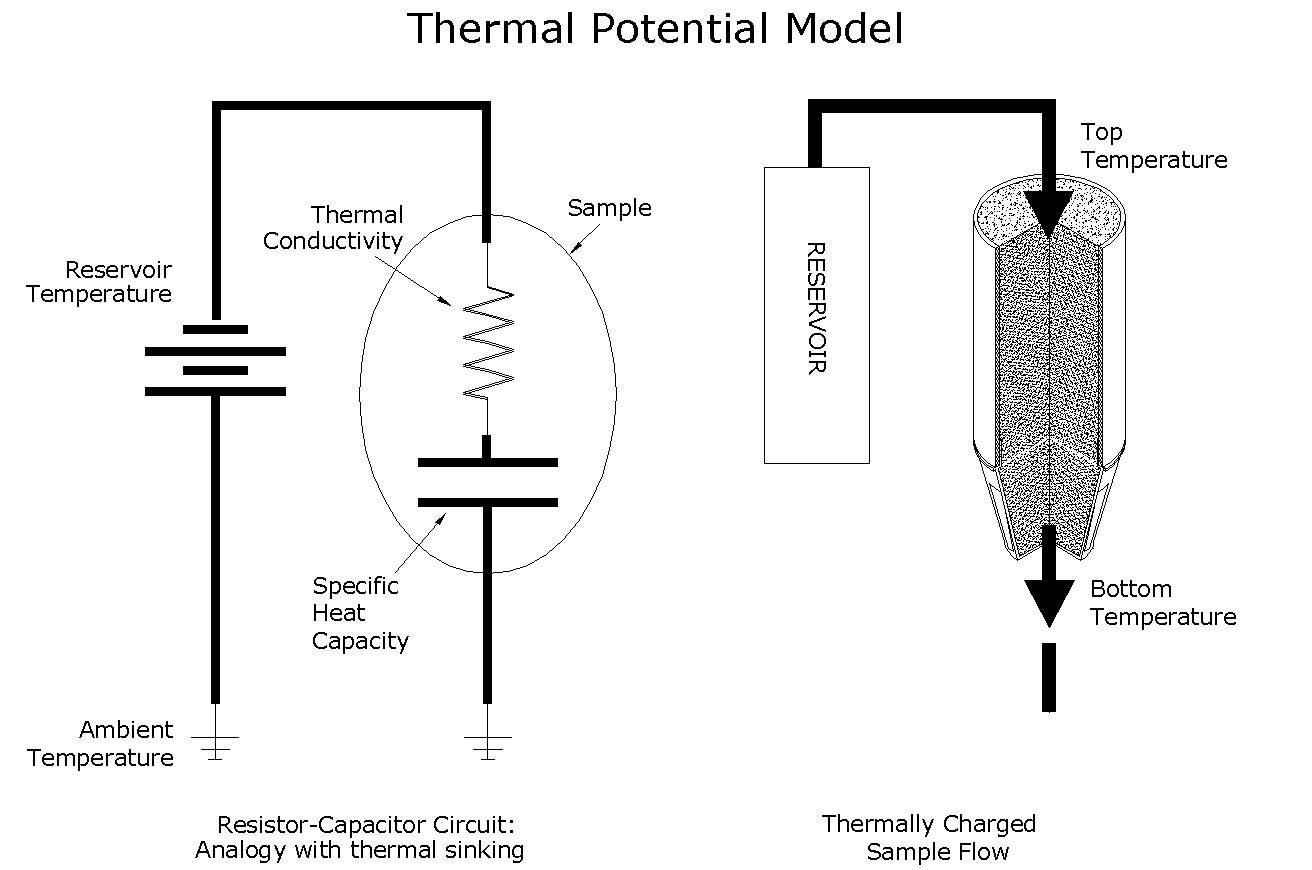
\includegraphics[scale=.35]{RCtherm.jpg}
\caption[Thermal Potential Model]{\textbf{\emph{The Potential Model Analogy}} An RC circuit is shown as a potential model for the sample vessel under thermal load. The net quantity of thermal energy transfered to the thermal sink inside the sample vessel is directly analogous to the capacitance of the RC circuit. The rate of that thermal energy exchange is a function of the thermal conductivity and the temperature difference that drives the exchange. These parameters are analogous to the resistance and applied voltage of the RC circuit.\label{rctherm}}
\end{center}
\end{figure}

Equation \ref{rc} and Figure \ref{rctherm} model the voltage across the capacitor as an RC \linebreak circuit charges \citep{elec}. In upholding the analogy, $V_{C}$ represents the temperature between the aggregate and the fluid flow at a time $t$. 

\begin{equation}\label{rc}
 V_{C}(t)=V(1-e^{\frac{-t}{RC}})
\end{equation}

The second part of this theory section realizes that the temperature gradient between the top and bottom temperature sensors at a time $t$ is not constant or linear, and consequently the temperature between the rock and the fluid will vary not only with time but also with position. Therefore, in applying the RC circuit analogy, $V_{C}$ must be interpreted specifically as the average, bulk temperature difference between fluid and aggregate. Any assumption that the temperture between the top and bottom locations is equivalent to the temperture difference between the water and the rock interface is oversimplified, and so this potential model serves only to describe the thermal sink effects on a bulk scale.

By Equation (\ref{rc}), using $V$ as the total available thermal potential, $T_{o}=T[TOP]-T[AMBIENT]$, substituting the thermal resistivity $\kappa^{-1}$ for $R$, $c_{R}$ as the capacitance $C$ and letting $\sigma$ represent a dimensional constant with units of $\frac{kg}{m}$, a thermal potential equation can be formulated from Equation (\ref{rc}):
\begin{equation}\label{rcNew}
T(t)[R]=T_{o}(1-e^{x})\:\:\:\:\:\:\:x=\frac{\sigma t}{\left[\frac{c_{R}}{\kappa}\right]}
\end{equation}

Figure \ref{rcthyplot} shows the thermal potential model of Equation \ref{rcNew} compared to data for two materials, QM1 and QM6. 

\begin{figure}[h!]

\begin{center}
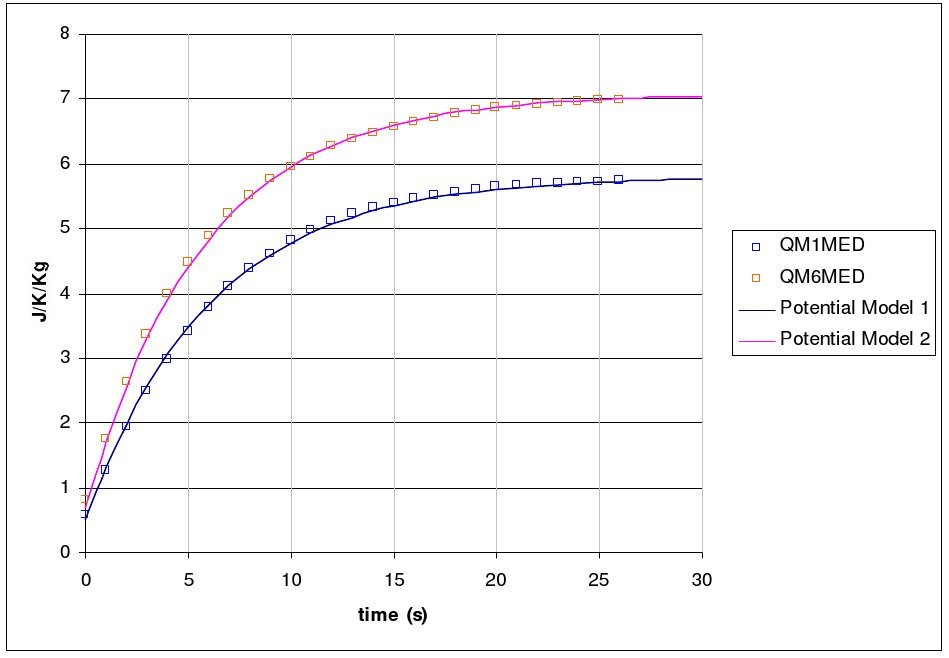
\includegraphics[scale=.4]{rcTheory.jpg}
\caption[Thermal Potential Data Comparison]{\textbf{\emph{A plot of a typical thermal potential model and a typical scaled, normalized CET plot}} Correlation coefficients for both plots was 0.98. Curves were optimized by plotting both dependent variables against one-another in a linear least squares regression model and fitting for a fixed $T_{m}$ value. Only the most extreme aggregate sizes were not well modeled by the thermal potential function, such as QM.3 and QM5 - refer to Figure (\ref{thMom}).\label{rcthyplot}}
\end{center}
\end{figure}

In the analysis of an RC circuit, the time constant $RC$ is used to characterize the response of the RC element. In the analog of that analysis, a new ``time constant'' appears in the exponent and is defined as the \emph{thermal moment}, $T_m$. 

\begin{equation}\label{tm}
T_m\;=\;\dfrac{\kappa}{C_R}
\end{equation}

This thermal moment characterizes how fast and how much heat can be transferred for an available potential, $T_{o}$. Let $\sigma=-\frac{R_{s}}{M_{s}}$ as necessary constants to compliment both $\kappa$ and $C_{R}$ and to dimensionally balance the exponent. 

\begin{equation}\label{rcExp}
x=\frac{\dfrac{R_{s}}{M_{s}} t}{\left[\dfrac{c_{R}}{\kappa}\right]}
\end{equation}

\begin{figure}[h!]
\begin{center}
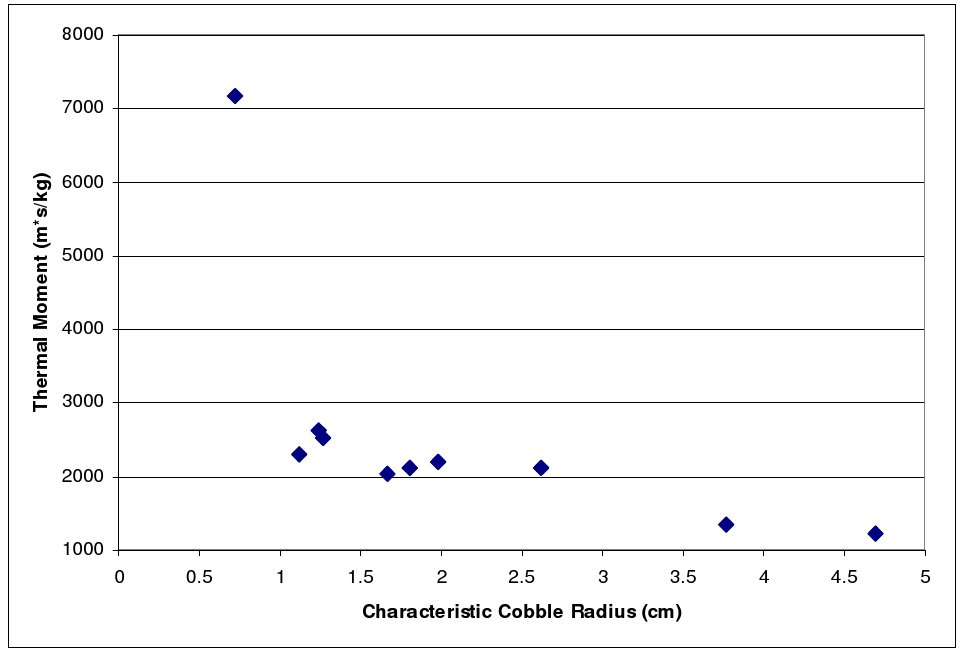
\includegraphics[scale=.4]{thMom.jpg}
\caption[Thermal Moment and Cobble Size]{\textbf{\emph{Thermal Moment and Cobble Size}} This illustrates a result from fitting both medium and low flow trials of the QM samples with Equation (\ref{rcNew}) and then extracting the exponent information to attain a thermal moment.\label{thMom}}
\end{center}
\end{figure}
\pagebreak
This new exponent, expanded in Equation (\ref{rcExp}) is a building block for a more detailed, empirical formulation of the heat exchange process. Unlike the RC circuit model however, flow considerations are taken into account. Additionally, there is one inconsistency of the analogy presented here  in the form of a floating ``boundary'' at the bottom temperature location compared to a grounded or absolute potential with the RC circuit. In the following emipirical formulation, this is taken into account to achieve what looks to be a much more accurate model, albeit with increased complexity.

\subsection{An Empirical Formulation from Experimental Parameters}

\begin{figure}
\begin{center}
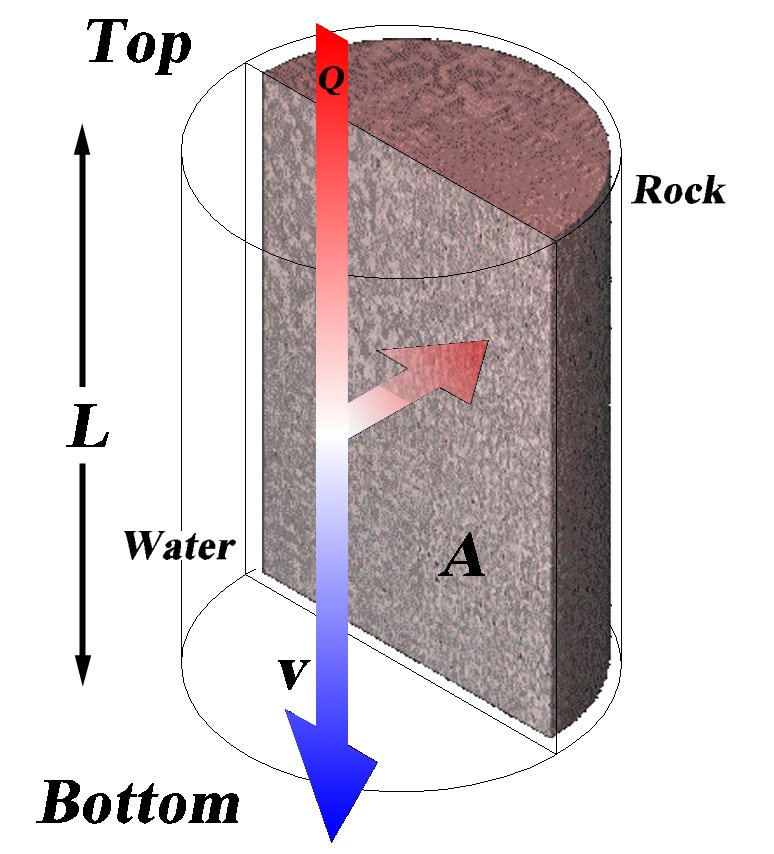
\includegraphics[scale=.25]{theorySlab.jpg}
\caption[Thermal Transfer Model]{\textbf{\emph{Thermal transfer inside the heat exchange vessel}} A simplified model of the gravitationally charged experimental sample vessel where heat is exchanged between a hydraulic flow (water) and a thermal sinking sample (rock - aggregate). This model, along with Fourier's Law, serves as the basis for the formulation of a cobble-level heat exchange model that draws its parametrization from data.\label{slab}}
\end{center}
\end{figure}

The method that follows is currently being developed by C.S. Thaxton as a means of providing a theoretical understanding of the heat exchange processes in aggregate materials. The work here is presented as a theoretical base that was derived from and ultimately supported by the data collected in this experimentation.

The experiment can be theorized in a general scenario that is founded on Fourier's Law, and does not depend on the sample or test material being of a un-consolidated nature. In this scenario, the test material is modeled as a solid slab for simplicity in determining a thermal contact area $A$ and in considering a flow regime. Furthermore, all heat transferred is assumed to take place only through a conduction mechanism, and convective or radiative processes are not considered in this formalism \citep{theoryKern}.

\noindent At any differential vertical segment $dl$, Fourier's Law is approximated as the following:
\begin{equation}\label{fouiers}
 \dot{Q}(L,t)=-\kappa A\;\frac{T(y,t)[W]-T(y,t)[R]}{R_{s}}
\end{equation}
Here, the aforementioned nomenclature holds, except instead of using a time-stepped temperature or energy value for numerical analysis, a differential is considered over both space and time, with $y$ representing a position along the sample's height. The gradient argument in Fourier's Law is assumed to be a finite distance between the water/rock interface and the center of the rock \citep{quench}. It is therefore represented by the rock's characteristic radius $R_{s}$. Solving this equation by means of variable separation and integration yields the following intermediate result.
\begin{equation}\label{Tbar}
\Delta Q_{net}=-\kappa\left(\dfrac{A}{R}\right) \int_{0}^{t_{f}} \left[ \dfrac{1}{L}\int_{0}^{L} T[WR](y,t)dy \right]dt\:=\:-\kappa\;\frac{A}{R}\int_{0}^{t_{f}}\bar{T}[WR](t)dt
\end{equation}
Where the bracketed term is the spatial average of $T(t)[WR]$ along $L$ and is numerically equivalent to Equation (\ref{rt}):
\begin{equation}\label{spatialT}
 \bar{T}(t)[WR]=\frac{1}{L}\int_{0}^{L}T(y,t)[WR]dL\;=\;\dfrac{-\Delta T(t)[TB]}{\sum\Delta T(t)[TB]}\left(2T[TOP]-T[AMBIENT]\right)
\end{equation}

By considering the first law of thermodynamics and net heat transfer as was discussed in the experiment section, it's possible to theoretically arrive at the following differential equation \citep{theoryKern}:
\begin{equation}\label{tempdiffeq}
 \dot{T}(y,t)[WR]=-\frac{\kappa(c_{R}-c_{W})}{C_{R}\;c_{W}}\frac{A}{R}\;T(y,t)[WR]
\end{equation}
This is soluble with the following function:
\begin{center}
\begin{equation}\label{solution}
\begin{aligned}
 T(y,t)[WR]=&T(y,0)[WR]e^{-\sigma_{f} t}\\
 \sigma_{f}=&-\frac{A(C_{R}-C_{W})}{R_{s}C_{W}}\;T_m\\
 T_m=&\frac{\kappa}{C_{R}}\\
\end{aligned}
\end{equation}
\end{center}
Equation (\ref{tempdiffeq}) can be simplified by letting $y=L$ and considering just the bulk temperature change over the entire sample and by assuming that the intial temperature difference between water and rock is equivalent to the total available potential difference between reservoir and ambient temperatures \citep{theoryKern}, let $T(0)[WR]=T_{o}$:
\begin{equation}\label{tempdiffeq2}
 \dot{T}(t)[WR]=T_{o}e^{-\sigma_{f} t}
\end{equation}

This solution is aligned with the result from the Thermal Potential Model. Understanding how various parameters in each of the respective exponents needs to be studied. The exponent in the Thermal Potential Model appears over simplified and the curve only matches well behaved or ideal energy transfers. The aforementioned empirical theory expands to include another exponential term that accounts for interaction area of the flow and rock, in addition to flow rate. 

The plots in Figure (\ref{steelHigh}) demonstrate that the empirical thermal model is directly consistent in predicting a vessel temperature differential by computing the temperature gradient as a function of length and time. However, more complex predictions fail to generate real values due to an inability to scale the flow and contact area parameters accurately. Because this supporting theory is still being developed, future research should seek to understand more exact parametrizations, especially with respect to flow and contact area.

This empirical model also introduces a second exponential term, consistent with a more general solution to the heat equation, and capable of accounting for flow related variables.
\begin{equation}\label{completetemp}
\begin{aligned}
\bar{T}[WR](y,t)=&\frac{1}{\beta L}T[WR](0,0)\;e^{-\alpha t}(1-e^{-\beta L})\\
\beta=&\left[\frac{C_{R}-C_{W}}{C_{R}\;C_{W}}\right]\;\frac{\kappa A}{\nu R_{s}}
\end{aligned}
\end{equation}


\begin{equation}\label{completeheat}
\begin{aligned}
Q_{net}=&Q_{0}-\frac{\gamma}{\alpha}(1-e^{-\alpha t})\\
\gamma=&\;\frac{\kappa A}{R_{s}}\frac{1}{\beta L}\;T[WR](0,0)(1-e^{-\beta L})
\end{aligned}
\end{equation}

\pagebreak

\begin{figure}[!h]
\begin{center}
\caption[Empirical Model and Data Comparison - Low]{\label{steelMed}}
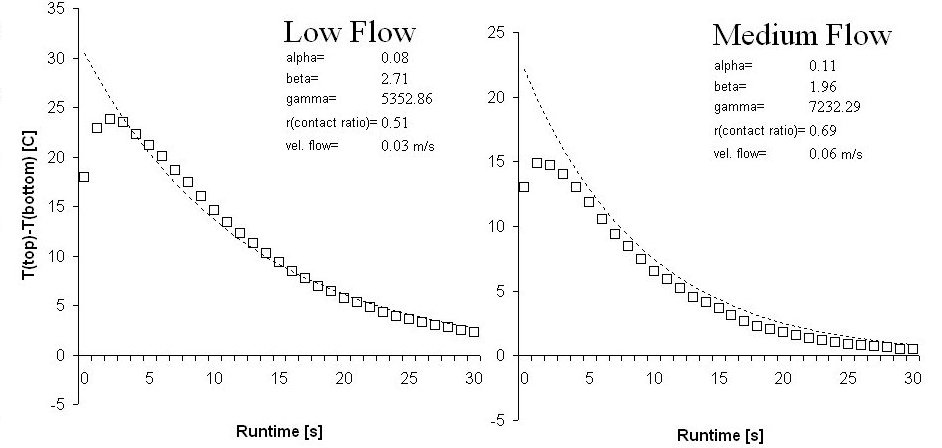
\includegraphics[scale=.5]{flowDouble.jpg}
\end{center}
\end{figure}

\begin{figure}[!h]
\begin{center}
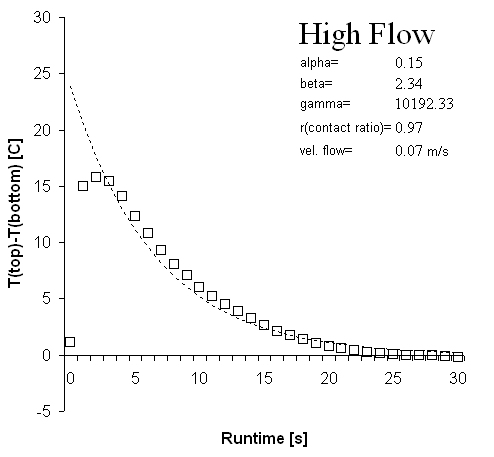
\includegraphics[scale=.5]{steelhighFlow.jpg}
\caption[Empirical Model and Data Comparison - High]{\textbf{\emph{Empirical model results vs. experimental temperature differences}} The empirically derived model successfully predicts the temperature difference across the vessel on a control sample of mild steel balls across a range of flows. The time and length dependent temperature gradient that defines the vessel heat exchange is part of this model. The flow rates are 0.25, 0.43 and 0.55 L/s, respectively.\label{steelHigh}}
\end{center}
\end{figure}
\pagebreak

%%This file will be included in the ThesisMain Document as the experimentation
%section.

%Author: James Kelly
%Last Modified: 11-12-08

\begin{center}
\section{Discussion and Results}
\end{center}

The fundamental motivation for this experimentation was first and foremost to quantify the thermal sink capacity of a bulk aggregate. Additionally, results should demonstrate that a mass of such material can and will remove a measurable amount of thermal energy from a thermally charged flow. Any result short of this hypothesis would effectively render the implementation of aggregate material ineffective as a solution to thermally charged stormwater discharge. Some material comes close to being thermally inert with respect to removing adequate amounts of thermal energy from a hydraulic flow. However, most material has demonstated some capacity to sink a thermally charged flow.
 
It is especially noteworthy in the case of most of the tested materials, given the relatively small thermal heat capacity and thermal conductivities, that the quantity and rates of heat were observed. The experiment was conceived on the hypothesis that aggregate materials were incorrectly assumed to have significant thermal sinking effects. Furthermore, some samples offer significant potential to relieve thermal duress under flow in severe scenarios, if implemented properly. It is therefore the goal of this discussion to consider the data and provide a foundation for further research and insight into using un-consolidated materials - of any form - to thermally sink a hydraulic discharge.

\subsection{Aggregate Parameters}

Several metrics are used in the performance analyses and ranking of the test materials. Bearing in mind that some of the materials were included in the experimentation strictly to diversify experimental results, several general conclusions can be stated with regard to completely practical materials. This section discusses these metrics and explains their role in the evaluation of an un-consolidated material's thermal sink performance.

Specific intrinsic parameters were identified and used to guide experimentation. Additionally, several environmental variables were also identified and used likewise. The choice of these parameters was based on the expectation that a respective variation would have a measurable effect on the thermal sink capacity of the sample aggregate. Several of these parameters were not directly measured or included in the current analysis primarily because they exceeded the intended scope of the experiment and available resources. However, results from theoretical renderings indicate some of these untested parameters may play an important role in an aggregate's thermal response. Some of these parameters include porosity, fineness modulus, isotropy, Mohs hardness and cobble geometry. For the purposes of this discussion, such parameters have been ruled as having only peripheral effects compared to more dominant parameters such as cobble size, bulk density and composition, and are consequently not part of this analysis. Continuing experimentation should investigate possible thermal relationships with these characteristics. 

Parameters that were isolated and studied for their contribution toward any sort of thermal response in a sample are listed in Table (\ref{matrix}). In considering material based characteristics, all tested aggregates share a comparatively narrow range of thermal properties given that they are all some sort of rock \citep{heatxfer}. Material is the single most dominant characteristic with respect to heat capacity $C_{R}$ and thermal conductivity $k$. That is to say that if a material with twice the heat capacity and thermal conductivity is used, a similar change in cobble size will have much less of an effect. This result was confirmed with the testing of both glass and steel balls in comparison to aggregate materials. In generalizing the results beyond aggregates, it is necessary to bear this in mind. However, in the regime of aggregate materials, the dominant variable that emerges is cobble size, because the materials are all quite similar with respect to $c_{R}$ and $k$. 

\begin{table}[t] 
\centering                           
\caption[Thermal Sink Parameters]{Thermal Sink Parameters: These intrinsic parameters were isolated and used to direct experimentation and theory and are listed in their order of their measured contribution to thermal sink capacity.\label{matrix}} 
\begin{tabular}{l l}           
\\[1ex] 
\hline\hline             
Intrinsic Parameters
\\
\hline 
\\
Material\\
Characteristic Radius\\
Mass\\
Packing Fraction\\
\\
\hline\hline
Systemic Parameters\\
\hline
\\
Flow Rate\\
Initial Flow Temperature\\
\\
\hline\hline
\end{tabular}
\label{tab:matrix}
\end{table}

Beyond using various types of aggregate to acheive a range of outcomes, reservoir temperature was varied slightly in addition to various flow rates. A variance in reservoir temperature did not change aggregate performance, but merely provided a basis for a thermal scaling of results. A ranking of aggregate thermal performance should be the same under any similar thermal potential and the total energy removed should also be the same. The time over which that energy is transferred to the aggregate will be exponentially slower with a decrease in the reservoir temperature. 

A variance in flow rate will naturally change the rate at which thermal energy is available for transfer. However, a varying flow rate also will affect the contact area between the flow and the aggregate surface area. This is true up to the point where the volume of fluid delivered to the aggregate in a period of time completely fills the interstitial space. At this point, the gravitationally driven flow will provide backpressure, and the aggregate will impose a different flow resistance. It is unknown if this scenario would present a different thermal transfer regime, as the available flow rates were always accommodated by the samples. The actual fraction of interstitial volume displaced by a known flow depends on several aggregate parameters, including geometry, packing fraction, porosity and surface interactions and overall fineness or cobble count. The fraction of interstitial volume displaced by flow can be estimated as follows:

\begin{equation}\label{flowDisp}
 Interstitial\:Flow\:Volume\:=\frac{I_{V}-\nu_{W}(t)}{I_{V}}
\end{equation}
\begin{equation}\label{sa}
Bulk\:Surface\:Area\:\approx\;4\pi R_{s}^{2}\;n\;M_{s}\left[\frac{nI_{V}}{V}\right]
\end{equation}
\begin{equation}\label{contact}
 Contact\:Area\;\approx\frac{Interstitial\:Flow\:Volume}{I_{V}}\:(Bulk\:Surface\:Area)
\end{equation}

In Equation \ref{sa}, the right hand term is a ratio that can be used to estimate the obliqueness of cobble geometry by accounting for the amount of interstitial space per cobble. Omitting this term would estimate a bulk surface area by assuming the cobbles are spherical. In Equation \ref{contact} the contact area is estimated as a real surface area, or by only considering the fractional part, as a ratio of the available surface area. This Equation includes several assumptions including the contact area between cobbles being negligible. Additionally, concavity of surfaces and porosity are not considered. 

\begin{table}[h] 
\centering                           
\caption[Contact Area Ratios]{Estimated contact area is expressed as a ratio with the available bulk contact area and is computed for each flow rate used in the experiment.\label{contactT}} 
\begin{tabular}{c c c}           
\\[1ex] 
\hline\hline
\\             
Flow Description & Flow Rate $\frac{L}{s}$ & Est Contact Area Ratio\\
\\
\hline
\\
Low & 0.20-0.30 & 0.18\\
Med & 0.35-0.45 & 0.23\\
High & 0.50-0.55 & 0.31\\
\\
\hline\hline
\end{tabular}
\label{tab:matrix}
\end{table}

In considering the flow through the vessel, we have not assumed any preferential flow patterns. The inflow has been observed to be very turbulent and the aggregate is randomly arranged such that there is little reason to suspect a highly preferential flow. However, larger cobbles such as QM5 and S2, and the steel and glass balls, have been thought to encourage more preferential flows, especially when noting their respective packing arrangements in the 4'' vessel. Specifically, a more voluminous flow along the walls of the vessel would bypass, to some degree, the main bulk of the sample. 

\subsection{Concepts of Thermal Sink Performance Metrics}

In reviewing the various parameters and related measures for rating the thermal sink performance of a particular un-consolidated material, it is pertinent to discuss how parameters affect or are affected by specific outcomes in the models and methods prescribed thus far. The following curves are plotted using the thermal potential model in Equation (\ref{rcNew}). In Figure (\ref{sinkComp1}) two samples with different specific heats and different thermal conductivities have been modeled. The ideal material possesses a thermal moment of $10\:\frac{kg}{m\bullet s}$ and the less responsive material possesses a thermal moment of $7\:\frac{kg}{m\bullet s}$. The ideal material has a much higher specific heat capacity and thermal conductivity, which is manifested in a steep ramp to its maximum J/K/Kg value. The ultimate amplitude of each curve is a direct result of the materials specific heat capacity, and the time until the curve reaches that level is a function of the thermal conductivity. The thermal diffusivity is not directly calculable from this information, as mass and bulk density directly affect it's value. If the slow response material were sufficiently lighter and less dense than the ideal sink material, the thermal diffusivity value could rate it higher.

\begin{figure}
 \centering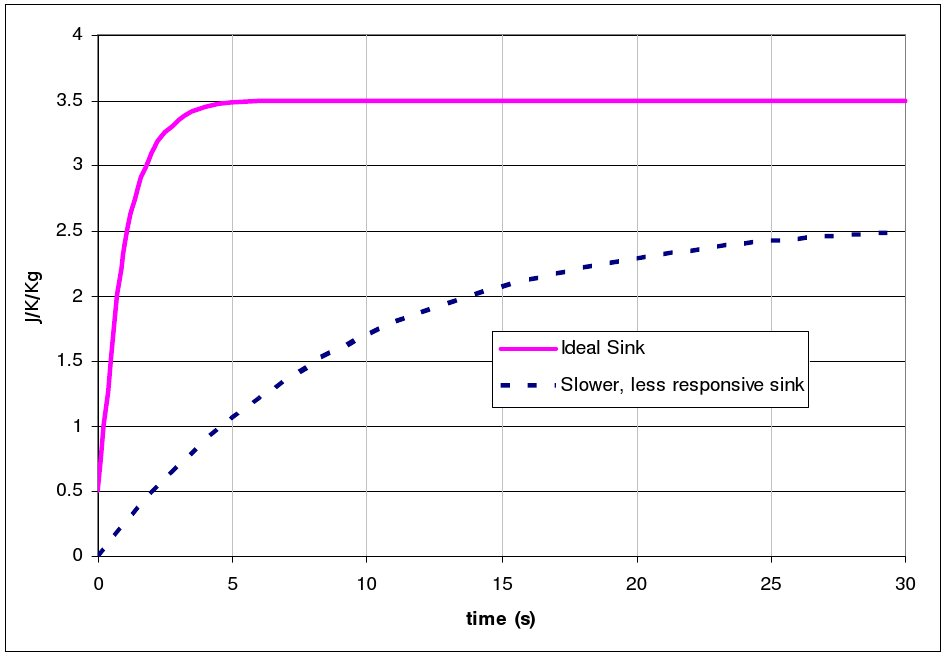
\includegraphics[scale=0.5]{sinkComp1.jpg}
 \caption[Theoretical Heat Sink Performances]{\textbf{\emph{Comparison plot of an ideal and low performance heat sink}} This model illustrates two materials of varying specific heat and thermal conductivity sinking thermal energy.\label{sinkComp1}}
\end{figure}

In this comparison, it's most important to note that no single parameter can summarize the complete thermal sink performance of a particular aggregate.

\subsection{Interpreting the Scaled, Normalized CET Function}
In graphically comparing different materials' trials with one another, the Scaled Normalized Cumulative Energy Transfer (CET) Function (SNCET) (Eq \ref{SNSCF}) was scaled by the measured heat capacity of the respective trial to yield a function with dimensions J/K/kg. This is a function that graphically illustrates the rate at which energy was exchanged with an amplitude that is analogous to the net energy transferred between water and aggregate. 
\begin{equation}\label{SNCSF}
 SNCET(t)\;=\;\dfrac{\Delta T(t)[TB]}{\sum\Delta T(t)[TB]}(c_{R})
\end{equation}
The primary purpose of creating a SNCET plot is to rank or compare different aggregate trials. It is a way to visualize and compare thermal sink performance amongst other aggregate families. Plots of the actual energy exchanged are listed in Appendix C, series 2. Shown is a SNCET plot of all medium flows in Figure (\ref{med1}). This plot serves to partially demonstrate the dominance of material over cobble size, noting how both SB1 (steel balls) and GB1 (glass balls) are 1'' in diameter with nearly identical characteristic radii. In aggregate trials, a comparable change in characteristic radius does not yield equally as dramatic differences in the SNCET plot. Additionally, noting how the aggregate materials have similar specific heats compared to SB1 and GB1, the most variance is a result of cobble size. 

In Figures \ref{med1} and \ref{low1}, each plot features several Scaled, Normalized Cumulative Energy Transfer (SNCET). Drawing from the aforementioned model in Figure \ref{sinkComp1}, several specific thermal sink characteristics can be interpreted. The rate of the function's rise to its maximum asymptote can be visually interpreted as the rate at which thermal energy is transferred into the aggregate mass, otherwise realized as the thermal conductivity. The value of the maximum asyptote is directly attributable to the heat capcity of the aggregate. As is argued with the thermal moment, $T_m$, both parameters need to be considered in rating a particular thermal sink performance. Generally, for maximum mitigation in an application, a large heat capcity is needed, but also at least a moderate to high thermal conductivity. The aggregates that offer the most promising SNCET are QM1 and QM6. 

\begin{landscape}
\begin{figure}
\vspace{4mm}
 \centering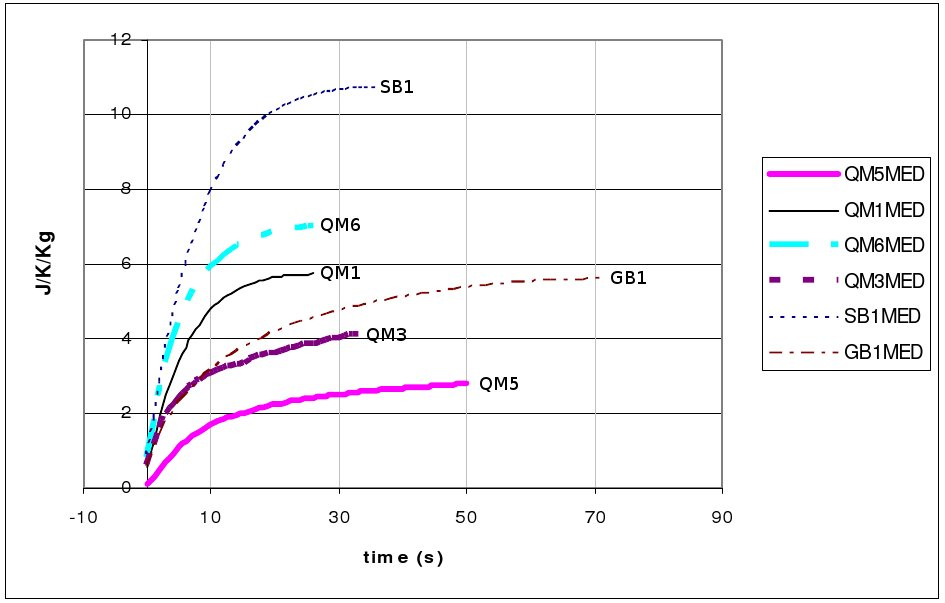
\includegraphics[scale=0.7]{med1.JPG}
 \caption[Scaled, Normalized CET - Medium Flow]{\textbf{\emph{Scaled, Normalized Cumulative Energy Transfer Function from medium rate trials}} Each trial is comparable in both a rate and quantity of thermal energy transfer under a medium flow rate.\label{med1}}
\end{figure}
\end{landscape}
\begin{landscape}
\begin{figure}
\vspace{4mm}
 \centering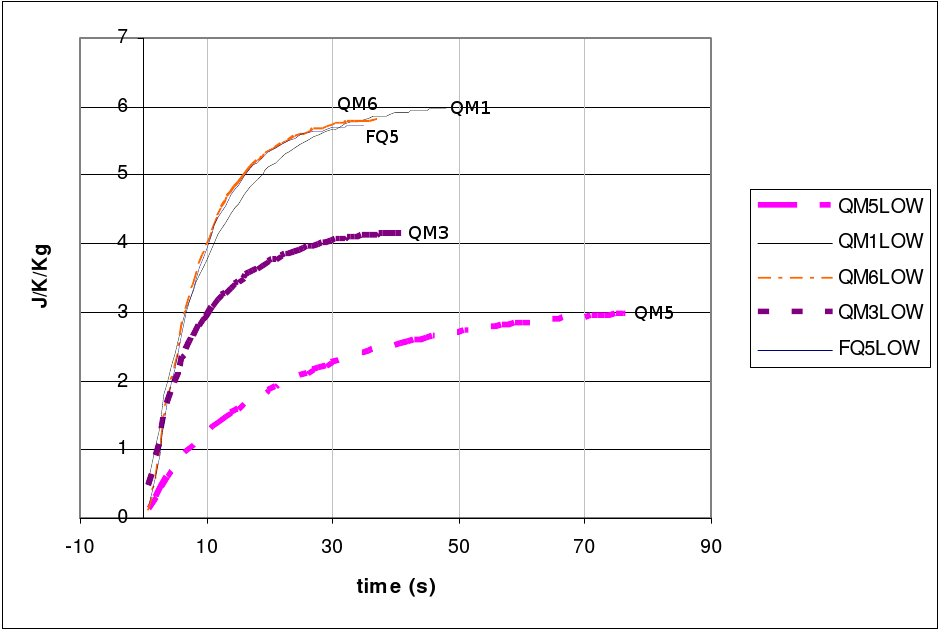
\includegraphics[scale=0.7]{low1.jpg}
 \caption[Scaled, Normalized CET - Low Flow]{\textbf{\emph{Scaled, Normalized Cumulative Energy Transfer Function from low rate trials}} Each trial is comparable in both a rate and quantity of thermal energy transfer under a low flow rate.\label{low1}}
\end{figure}
\end{landscape}
In Figure (\ref{med1}) two samples, QM.3 and QM5 offer thermal sink performances less than the glass balls. Each of these samples represent the extreme cobble sizes used in the experiments at 0.375'' and 5'', respectively. Noting how the mid-range cobble sizes offer both faster sink rates and total energy transferred during the trial, Figure (\ref{opt1}) demonstrates that there is an optimal cobble size for a given set of flow conditions. Note that this plot uses a maximum SNSCF value, so that this is actually expressing the total amount of energy that was transferred for a normalized temperature difference. Two different flows are depicted in Figures (\ref{med1}) and (\ref{low1}) - a medium and a low flow rate, for comparison. The flow rate seems to be a secondary parameter that stands to increase or decrease the amplitude of the curve while the cobble size will shift the peak of the curve left or right. 

\begin{figure}[h!]
\centering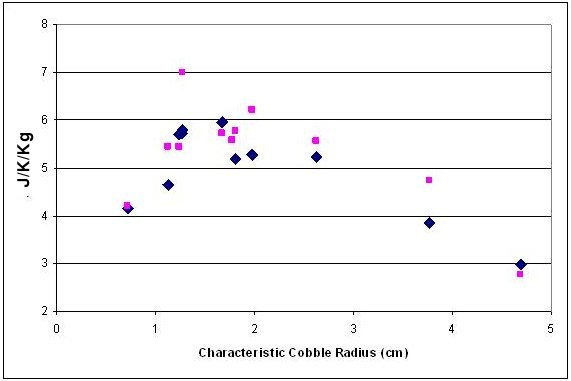
\includegraphics[scale=0.6]{opt2.JPG}
\caption[Scaled, Normalized CET vs Cobble Size]{\textbf{\emph{SNCET (J/K/Kg) versus cobble size - }} This plot shows an optimal cobble size under certain flow conditions. A low flow rate is represented by the diamond symbols, and a medium flow rate is represented by the squares.\label{opt1}}
\end{figure}

In studying this trend, the data indicate that as the flow rate increases, the optimal cobble size for thermal sink response should decrease slightly. This is intuitive, knowing that the larger cobbles possess a slower thermal response due to their bulk, and a lower flow can accomodate this best. A higher flow rate - and in turn a higher thermal wattage imparted on the aggregate -  will demand a faster thermal response than a smaller cobble could provide. There are, however, flow considerations to bear in mind as well, noting that a decrease in cobble size restricts flow, so in turn there is an optimization boundary. 

Hybrid aggregates warrant testing based on these results. It is conceivable that an aggregate of two or more different cobble sizes could offer both flow and thermal sink capacity with some compromise in total bulk. A preliminary analysis of a thermal sink capacity of such a material could be formulated from the current data. However, flow mechanics, the packing ratio and thermal contact parameters will naturally be different with hybrid aggregate, and so the exact results are not directly predictable from the current data.

\subsection{Thermal Conductivity, Moment and Diffusivity as Performance Indicators}
Thermal conductivity $\kappa$ is an intrinsic characteristic directly related to the material of the aggregate. It simply conveys the rate at which heat is transferred through the material, and it is the usual proportionality constant in modeling thermal energy transfers with the heat Equation. Thermal conductivity, as discussed in the experimentation section, is calculated from the data sets and then used to arrive at the thermal diffusivity. A high specific heat, sufficiently large cobble size and high thermal conductivity will help ensure that the aggregate can afford to remove more heat per unit time. 

The thermal moment, previously defined as $T_{m}=\frac{\kappa}{c_{R}}$, demonstrates that it is an important characteristic in the modelling of an aggregate's thermal response. In the experimental calculations, cobble size was embedded in the thermal conductivity as the gradient length, and therefore cobble size is inherent in the $\kappa$ values listed in this experiment. Ideally, $\kappa$ should compute to be the equal across the same material, but initial numerical calculations demonstrate a significant variance. This indicates that the cobbles are thermally loaded faster than the $\kappa$ calculations are assuming. According to Clauser \citep{kRocks}, quartzite has $k=7.7$ and the average for all quartzite cobble sizes used in experimentation is $k=10.5$. 

Thermal diffusivity is a quantitative measure for a particular mass's ability to respond to a thermal change in its environment. The lower the thermal diffusivity, the less thermal response per unit mass the sample will have. Diffusivity was computed in an attempt to arrive at some bulk unitary index with which to rate an aggregate, independent of flow. It is computed using bulk density and, of course, bulk temperature differentials, and so it should reflect the response of the entire aggregate mass as a whole. This is said with the assumption that a mass of aggregate will behave differently under duress when compared to a single cobble or material isolate.

%\paragraph{Power Analyses of Thermal Sink Capacity on a Themally Charged Creekflow}

%Optimally, $1-m^{3}$ of 1'' aggregate can produce up to 1000-kW of thermal sink power. A medium sized creek during a rain %event can be estimated at 3000-5000-kW at a peak flow rate of about $3-m^{3}$. 

\subsection{Recommendations for Thermal Buffering of Watersheds}

Temperature Total Maximum Daily Load (TMDL) regulations are imposed at both federal and state levels in select or sensitive waters that are subject to thermal charging from development, urban surfaces or industry \citep{urban}. Using construction aggregate for thermal buffering is only suitable where a small amount of energy needs to be removed from the flow. This could either be manifested as a short but dramatic rise in temperature levels from a point source or tributary or a small temperature change over a more prolonged period of time. The scope of this experiment was an investigation of point source mitgation under severe thermal duress for short periods of time. It is not reasonable to extrapolate these results to   time frames of more than a few minutes, especially if the aggregate is not enclosed. Convective and radiative heat loss will stand to yield much different thermal sinking effects if temperature differences are small and time frames are long.

Engineering solutions that currently implement aggregate as a thermal buffer typically lay the aggregate out in a piled mass to fill an entrenchment or drainaige basin that catches discharge before it is released into the watershed. In such scenarios, it can be stated that if there is known thermal spiking in the discharge, the aggregate will remove some thermal energy. However, analytically, flow patterns in piled gravel are not optimal for thermal sinking. In implementing an aggregate thermal sink, the following generalizations have been derived from the data:

\begin{itemize}
 \item Use of a medium sized cobble is preferred to allow sufficient flow, a minimum maintenance schedule and maximum thermal sink effects. These studies suggest $R_s=1-3\;cm$ for the flow rates measured.
 \item Arrangement of the aggregate such that the flow contacts as much of the available surface area as possible: Shallow surface arrangements, aggregate filled pipes or culverts, and baffles or flow vanes to redistribute the flow to other parts of the aggregate are all measures that could be taken to ensure maximal thermal contact area under flow.
 \item If a known point source exhibits thermal charging and its total thermal overload can be estimated in terms of a net energy difference, then for every unit volume of water that needs to be reduced by 1 degree, approximately that same volume of aggregate should be implemented to sink the flow. This is based on the assumption that the temperature differences between the aggregate and the overloaded water are greater than about 10 degrees. 
 \item For every unit volume of aggregate used, the thermal response of the creek will be damped by a factor proportional to the thermal moment of the aggregate and equal to the exponent in Equation (\ref{solution}). A simple analysis of this result can be visualized in the thermal sink power of the aggregate. If a thermally charged flow ramps with a known increase in flow rate and temperature, the thermal sink power of an ideally situated aggregate can be subtracted from the change in the discharge power to yield a reduced thermal acceleration or damping of the temperature spike. It should be stated that this is only a reasonable expectation for thermal sinking as the volume of aggregate needed to literally reduce the effective temperature increase by a few degrees in a storm induced flow is on the order of $10^{3}-m^{3}$ for even a very small creek.
 \item The maximum thermal sink power observed for an entire trial period in a common aggregate was 4-kW. Based on flow rate and thermal overloading conditions, this maximum sink power can be considered only under graviationally charged flow with no pressure head and less than 50\% flow capacity of the aggregate. Total immersion in a flow will only reduce this thermal sink power. 
\end{itemize}

\subsection{Conclusion}
Ultimately, the emphasis on using aggregate to thermally sink a thermally charged flow is to only damp a rapid change in temperature. The net change in temperature can only be artificially managed by eliminating or reducing thermal charging at the source or infiltration. 

Aggregates act to store heat for later release - damping the thermal spikes inherent to point sources. The effectiveness of this process is dictated primarily by (i) material composition, (ii) size, (iii) total mass, and (iv) packing fraction. The governing thermal parameters of the aggregate materials available on construction sites all fall within a narrow range such that the ideal solution would likely be a mixture of different materials and sizes small enough to retain the heated water for cooling while large enough to allow flow under large rain events. In addition, closed aggregate solutions in thermal contact with the earth would likely improve the thermal sink performance of the aggregate. Engineering solutions would have to be designed based on anticipated flow rates, overall discharge volumes, availability of aggregates, and ease in clean-out maintenance. This study clearly shows that effective thermal buffering can be achieved with such designs for small mountain streams exposed to flashy thermal charging.

%\bibliographystyle{} %Unabbreviated references with article titles (manuscript format)
%\bibliography{references}

%\appendix
%%Author: James Kelly
%Last Modified: 10-26-08
\doublespacing
\section*{}
%\begin{table*}[h]
\centering
\subsection*{A-1: Nomenclature}
%\caption{\label{nom}Definitions of Sample Parameters} 
\textbf{Definitions of Sample Parameters}\\[4mm]                          
\begin{tabular}{c | c| c| c}           
\hline\hline
Parameter	& Units				&Description & Source\\
\hline
V		&Liters& Sample Vessel Volume	& Measured\\ %/ Fluid Displacement $\pm 5-cm^{3}$\\
\hline
   
n		& &Number of Cobbles or Grains	& Measured\\ % / Counted and Inferred $\pm 1\%$\\
\hline
   
$R_{s}$		&cm&Characteristic Radius 	& $R_{s}=\left[\tfrac{3(V-I_{V})}{4n}\right]^{\tfrac{1}{3}}$\\
\hline
   
$M_{s}$		&kg& Sample Mass 		& Measured\\% / Scale $\pm 0.2 kg$\\
\hline
   
$\rho_{s}$ 	& & Sample Specific Gravity	& $\tfrac{M_{s}}{V-I_{V}(\rho_{H_{2}O}}$\\
\hline
   
$\rho_{bulk}$	&$\tfrac{kg}{m^{3}}$&Bulk Density& $\tfrac{M_{s}}{V}$\\
\hline
   
$I_{V}$		&Liters&Interstitial Volume	& Measured\\ % / Fluid Displacement $\pm 5-cm^{3}$\\
\hline
   
$\tfrac{V_{s}}{V}$& &Packing Fraction		& $\tfrac{V_{s}}{V}=\tfrac{V-I_{V}}{V}$\\
\hline
   
$\tfrac{n}{kg}$	& &Cobble Count			& Measured\\ % / Count per 1 kg $\pm 1\%$\\
\hline
   
$k$		&$\tfrac{W}{m\dotfill K}$ &Thermal Conductivity &\\
\hline
   
$k_{s}$		&$\tfrac{W}{m\dotfill K}$ &Bulk Thermal Conductivity & Computed\\% / Refer to Theory Section\\
\hline
   
$c$		&$\tfrac{J}{kg\dotfill K}$ &Specific Heat &\\
\hline
   
$c_{s}$		&$\tfrac{J}{kg\dotfill K}$ &Bulk Specific Heat & Computed\\% / Refer to Theory Section\\
\hline
   
$\alpha$ 	&$\tfrac{m^{2}}{s}$ &Thermal Diffusivity & $\alpha=\tfrac{k}{\rho_{s}c}$\\
\hline
   
$\alpha_{s}$ 	&$\tfrac{m^{2}}{s}$ &Bulk Thermal Diffusivity & $\alpha_{s}=\tfrac{k_{s}}{\rho_{bulk}c_{s}}$\\
\hline\hline
\end{tabular}
%\end{table}
\vspace{6mm}

Note that all parameters listed here are computed directly from data.









 
%%This file will be included in the ThesisMain Document as the copywright page.

%Author: James Kelly
%Last Modified: 10-08-2008

\doublespacing
\section*{}
\thispagestyle{empty}       %do not display page numbers
\begin{center}
\begin{Large}
\vspace{50mm}
\subsection{Sample Aggregate Statistics}
\vspace{6mm}
\subsubsection{Nomenclature}
\subsubsection{Sample Table}
\end{Large}
\end{center}

%\includepdf[pages=-,landscape=false]{samples.pdf}
%\vspace{10cm}
%\begin{center}
%\section{Flow Sensor DAQ Source Code}
%\end{center}

%What follows is the source code used to build the flow sensor data acquisition front panel. This code is to be run in a Visual %Basic Compiler, specifically VB 5.0 or 6.0 using a Win98 operating system. This code requires that RSTimer be installed in the %Visual Basic Environment. Additionally, parallel port addresses and ports should be aligned and set in the code before use.

%\pagebreak
\begin{singlespace}
\begin{small}
\begin{verbatim}
'Flow Sensor Interface V2
'Written by James Kelly
'Surface and Terrestrial Processes Lab
'April 2008
'
'This is an interface driver that reads data from LPT1
'on Data Pin 1 from a rotary flow sensor.

'RSTimer1 is for time stamp generation at 0.1 sec resolution
'RSTimer2 is for frequency calculation at 1 sec resolution
'RSTimer3 is for edge counting from the flow sensor signal at 1ms resolution
'RSTimerFlow is for flow specific time management only during flow events

Option Explicit

'Subs to establish Parallel Port commands
Private Declare Sub vbOut Lib "WIN95IO.DLL" 
(ByVal nPort As Integer, ByVal nData As Integer)
Private Declare Sub vbOutw Lib "WIN95IO.DLL" 
(ByVal nPort As Integer, ByVal nData As Integer)
Private Declare Function vbInp Lib "WIN95IO.DLL" 
(ByVal nPort As Integer) As Integer
Private Declare Function vbInpw Lib "WIN95IO.DLL" 
(ByVal nPort As Integer) As Integer

'output data arrays
Private flowData() As Double
Private timeData() As Double
Private timeStamp() As String
Private cumFlowData() As Double

'timekeeping vars
Private msec As Long, sec As Long, min As Long, hr As Long
Private fmsec As Long, fsec As Long, fmin As Long
Private tStmp As Double
Private fTime As Double, calibrationConst As Double

'operating flags
Private outToggle As Boolean
Private activeFlag As Boolean, launchTim As Date, flowON As Boolean
Private saveFlag As Boolean

'sampling vars
Private i As Long
Private freqCount As Double
Private edgeDetect As Integer, deltaEdge As Integer
Private cumF As Double, currF As Double

'File and calibration vars
Private volume As Double
Private portNumber As Integer
Private Units As Boolean 'Imperical = False, Metric = True



'Front Panel Initialization
Private Sub Form_Load()

activeFlag = False

'Clock intialize
msec = 0
sec = 0
min = 0
hr = 0

'flow clock initialize
fmsec = 0
fsec = 0
fmin = 0

tStmp = 0
et.Caption = "0:0:0.0"
sr.Text = "1"
cf.Caption = "0"
lt.Caption = ""
ft.Caption = ""
cumFlow.Caption = "0"
flowON = False
currF = 0
cumF = 0
cConstant.Text = "0.005766"
cmdStop.Enabled = False
cmdReset.Enabled = False
saveFlag = True
portNumber = 957

'initialize frequency measurement vars
edgeDetect = 0
deltaEdge = 0
freqCount = 0

'Intialize intervals of timers
RSTimer1.Interval = 100     '0.1 sec
RSTimer2.Interval = 1000    '1 sec
RSTimer3.Interval = 1       '1ms
RSTimerFlow.Interval = 100
RSTimerFlow.Enabled = False

End Sub
'Launch for DAQ
Private Sub cmdLaunch_Click()
        
        i = 0
        Call Reset
        
        RSTimer1.Enabled = True
        RSTimer2.Enabled = True
        lt.Caption = Time & "  " & Date
        activeFlag = True
        saveFlag = False
        flowON = False
        cmdCalibrate.Enabled = False
        cmdLaunch.Enabled = False
        cmdQuit.Enabled = False
        cmdStop.Enabled = True
        cmdReset.Enabled = True
        
        Do
        DoEvents
        If freqCount <> 0 Then
            
            RSTimerFlow.Enabled = True
            If flowON <> True Then fs.Caption = Time
            flowON = True
            
        End If
        If freqCount = 0 Then RSTimerFlow.Enabled = False
        Loop Until activeFlag = False
        
        cmdCalibrate.Enabled = True
        cmdLaunch.Enabled = True
        cmdQuit.Enabled = True
        cmdStop.Enabled = False
        cmdReset.Enabled = True

End Sub

'Time stamp generation
Private Sub RSTimer1_Timer()

'Nested If counts out for a time display
msec = msec + 1
If msec > 9 Then
msec = 0
sec = sec + 1
If sec > 59 Then
sec = 0
min = min + 1
If min > 59 Then
min = 0
hr = hr + 1
End If
End If
End If

'Double Int time stamp is computed for data handling
tStmp = sec + 0.001 * msec

'Assemble counters for time visualization
et.Caption = CStr(hr & ":" & min & ":" & sec & "." & msec)

'---Insert to test port 1 output response - must test ok at 1kHz---
'If outToggle = True Then
'vbOut 888, 0
'outToggle = False
'Else
'vbOut 888, 1
'outToggle = True
'End If

End Sub
'Timer for Freq calcuation at 1sec Resolution
Private Sub RSTimer2_Timer()

'Current Sample Flux Monitoring
ts.Caption = CStr(freqCount / CDbl(sr.Text))
'Reset sampling counter
freqCount = 0

'Compute Current Flow Rate
currF = 0.0164 * CDbl(ts.Caption) ^ 0.7504
'Display Current Flow
cf.Caption = CStr(currF)
If flowON = True Then

            'Compute Cumulative Flow
            cumF = currF + cumF
            'Display Cumulative Flow
            cumFlow.Caption = CStr(cumF)

            ReDim Preserve flowData(i)
            ReDim Preserve timeData(i)
            ReDim Preserve timeStamp(i)
            ReDim Preserve cumFlowData(i)
            
            RSTimerFlow.Enabled = True
            If flowON <> True Then fs.Caption = Time
            flowON = True
            
            'assembling data arrays for export
            flowData(i) = CDbl(cf.Caption)
            timeData(i) = i
            timeStamp(i) = Time
            cumFlowData(i) = CDbl(cumFlow.Caption)
            
            'visualization of data
            dataOut.Text = dataOut.Text & CStr(timeData(i))
		 & vbTab & Format$(flowData(i), "0.000") & vbCrLf
            i = i + 1

End If

End Sub
'Timer for edge counting of sensor signal at 1ms res
Private Sub RSTimer3_Timer()

edgeDetect = vbInp(portNumber)

If edgeDetect <> deltaEdge Then
    freqCount = freqCount + 1
    deltaEdge = edgeDetect
End If

End Sub

Private Sub RSTimerFlow_Timer()
'This is essentailly a duplication of the main elapsed time clock,
'but used for flow timing only.

fmsec = fmsec + 1
If fmsec > 9 Then
fmsec = 0
fsec = fsec + 1
If fsec > 59 Then
fsec = 0
fmin = fmin + 1
End If
End If

fTime = fmin + 0.016949152542 * fsec + 0.001 * fmsec

'Assemble counters for flow time visualization
If activeFlag = True Then fft.Caption = 
	CStr(fmin & ":" & fsec & "." & fmsec)
End Sub
'This resets display data and clears any data remnants in the output array.
'This is invoked manually or at launch time.
Private Sub cmdReset_Click()
Dim perg As Integer

If saveFlag = False Then
perg = MsgBox("Data has not been saved", vbOKCancel, "Data Purge?!")
    
    If perg = 2 Then Exit Sub

End If

lt.Caption = ""
et.Caption = ""
ft.Caption = ""
cf.Caption = ""
cumFlow.Caption = ""
ts.Caption = ""
fs.Caption = ""
fft.Caption = ""
fv.Caption = ""
dataOut.Text = ""
fmsec = 0
fsec = 0
fmin = 0

ReDim flowData(0)
ReDim timeData(0)
ReDim timeStamp(0)
ReDim cumFlowData(0)

saveFlag = True

cmdReset.Enabled = False

End Sub

Private Sub cmdSave_Click()

On Error GoTo DialogError

With CommonDialog1
    .CancelError = True
    .Filter = "Exported Data (*.dat)|*.dat"
    .FilterIndex = 1
    .DialogTitle = "Select a location and name for your data file"
    .ShowSave
End With

Dim c As Long
c = 0

Open CommonDialog1.filename For Output As #1

'Write data to filestream....
'Header info
Print #1, "ASU Surface and Terrestrial Processes Lab"
Print #1, "Stormwater discharge simulator flow sensor output"
Print #1, Date & timeStamp(0)
Print #1, comment.Text & vbCrLf
Print #1, "ElapTime (s)" & vbTab & "Current Flow" & 
		vbTab & "Cumulative Flow"

'dump flow data from arrays to filestream
Do
Print #1, timeStamp(c) & vbTab & timeData(c) & vbTab 
	& Format$(flowData(c), "0.00") & vbTab & Format$
		(cumFlowData(c), "0.00") & vbTab
c = c + 1
Loop While c < i

If c = 0 Then MsgBox ("No Data was Exported")

saveFlag = True
Close

DialogError:
If saveFlag = False Then MsgBox ("No Data was Exported")
End Sub

'Sub for creating a calibration curve and related linear constant
'Output calibration data is sent to a default flowCalibrate_x.dat file
'careful - this one's a mess!
Private Sub cmdCalibrate_Click()

'Calibration arrays
Dim flowDat() As Double
Dim timeDat() As Long
'For each variant variable
Dim flow As Variant
Dim timeD As Long
Dim sum As Double
Dim c As Integer, cc As Integer

Dim strVolume As String
Dim dataSave As Integer
    dataSave = 1
Dim sampleCnt As Long
    
cmdCalibrate.Enabled = False
cmdLaunch.Enabled = False
cmdQuit.Enabled = False
cmdStop.Enabled = True
cmdReset.Enabled = False

cConstant.Text = "1"
activeFlag = True
strVolume = InputBox("Enter Calibration Volume in Litres",
		 "Calibration Volume", "50")



If IsNumeric(CDbl(strVolume)) Then
    volume = CDbl(strVolume)
Else
    MsgBox ("Entered Value is not a number")
Exit Sub
End If
        
'management of existing data
If saveFlag = False Then dataSave = MsgBox("You may have unsaved data. 
	Cablibration will clear this. Continue?", vbOKCancel)
If dataSave = 1 Then
    saveFlag = True
    i = 0
Else
      Exit Sub
End If
        
RSTimerFlow.Enabled = True
        
        i = 0
        Call Reset
        
        RSTimer1.Enabled = True
        lt.Caption = Time & "  " & Date
        activeFlag = True
        saveFlag = False
        flowON = False
     
        Do
        DoEvents
        If freqCount <> 0 Then
            
            RSTimerFlow.Enabled = True
            If flowON <> True Then fs.Caption = Time
            flowON = True
            
        End If
        If freqCount = 0 Then RSTimerFlow.Enabled = False
        Loop Until activeFlag = False
        
    RSTimer1.Enabled = False
    RSTimer2.Enabled = False
    RSTimer3.Enabled = False
    RSTimerFlow.Enabled = False
    cmdEnable.Caption = "Timers Off"
    cmdEnable.Enabled = False

c = 0
cc = 0
sum = 0
dataOut.Text = ""

For Each flow In flowData
    If flow <> 0 Then
        ReDim Preserve flowDat(c)
        ReDim Preserve timeDat(c)
        flowDat(c) = flow
        timeDat(c) = timeData(cc)
        dataOut.Text = dataOut.Text & vbCrLf & timeDat(c) & 
		vbTab & Format$(flowDat(c), "0.00")
        
        sum = sum + flowDat(c)
                
        c = c + 1
    End If
    
    timeD = c
    
cc = cc + 1
Next
dataOut.Text = dataOut.Text & vbCrLf & "Time = " & CStr(timeD) & 
		vbCrLf & "Sample# = " & CStr(sum)

RSTimerFlow.Enabled = False

'calibrationConst = timeD / volume
calibrationConst = volume / sum
cConstant.Text = CStr(calibrationConst)
        
cmdCalibrate.Enabled = True
cmdLaunch.Enabled = True
cmdQuit.Enabled = True
cmdStop.Enabled = False
cmdReset.Enabled = True
        
End Sub
Private Sub cmdEnable_Click()

If (cmdEnable.Caption = "Disable") Then
    RSTimer1.Enabled = False
    RSTimer2.Enabled = False
    RSTimer3.Enabled = False
    RSTimerFlow.Enabled = False
    cmdEnable.Caption = "Timers Off"
    cmdEnable.Enabled = False
End If

End Sub

Private Sub cmdStop_Click()
RSTimer1.Enabled = False
RSTimer2.Enabled = False
activeFlag = False
flowON = False

        cmdCalibrate.Enabled = True
        cmdLaunch.Enabled = True
        cmdQuit.Enabled = True
        cmdStop.Enabled = False
        cmdReset.Enabled = True

End Sub
Private Sub cmdQuit_Click()
If saveFlag = False Then
MsgBox ("Data has not been saved. Please reset or save.")
Exit Sub
End If
End
End Sub
\end{verbatim}
\end{small}
\end{singlespace}
%%This file will be included in the ThesisMain Document as the copywright page.

%Author: James Kelly
%Last Modified: 10-08-2008
\section*{}
\doublespacing
\thispagestyle{empty}       %do not display page numbers
\begin{center}
\vspace{20mm}
\subsection{Data Plots}
\vspace{30mm}
\subsubsection{Quartzite Family}
\subsubsection{Marble and Brick}
\subsubsection{Siltstone, Cobble, Glass and Steel}
\subsubsection{Comparison Plots}
\end{center}
%\includepdf[pages=-,landscape=true]{plots2.pdf}
%\begin{center}
\section{Vita}
\end{center}
\thispagestyle{empty}
\linebreak

C. James Kelly was born in State College, PA to James P. and Mary Ellen Kelly. James has one sister, Megan who resides in State College, PA with her husband Ron and her new son, Ronald Patrick. James graduated from State College Area High School in June 1993 with a trade diploma in technical illustration and went on to work for the Office of Telecommunications at The Pennsylvania State University as an engineering assistant and draftsman. 

He graduated from Mansfield University of Pennsylvania with a BSE degree in Mathematics, while also fulfilling the requirements for the BSE degree in Physics. He completed two student teaching assignments, one at Southside High School in Elmira, New York under Mr. Charlie Wilson teaching Regents Physics, and one at Northern Tioga High School in Lawrenceville, Pennsylvania under Mrs. Cheryl Matteson teaching high school geometry. 

He then accepted a job teaching high school Math and Physics at Rockbridge High School in Lexington, Virginia. James successfully doubled the number of students enrolled in physics by his third year  and expanded a section of the school's precalculus course to be taught simultaneously with a section of introductory physics.

James accepted a position at Virginia State Polytechnic Institution and State University (Virginia Tech) in August 2005 as an instructor at the nationally recognized Math Emporium. 

James was married to Mary Dean Coleman in August of 2006, a PhD graduate of Virginia Tech, and the two then relocated to Boone, NC where Mary Dean accepted a faculty position. James was simultaneously accepted into the Engineering Physics graduate program in the department of Physics and Astronomy.

James is now relocating back to his hometown, where Mary Dean has accepted a professorship at The Pennsylvania State University. James hopes to pursue a technologically intensive research job. 

%Data
%\include{AppendixD} %Temperature Sensor Mods
%\include{AppendixE} %Flow Sensor Interface


%\bibliographystyle{astron} %Abbreviated references without article titles (article format)
%%The following document catalogs all the refence information. 

%Author: James Kelly
%Date Modified: 10-08-2008
\begin{thebibliography}{}
\bibitem[Bonner et al.(1977) Bonner, Fulford, and March]{Bonner77}
 R. F. Bonner, J. E. Fulford, and R. E. March, Int. J. Mass Spectrom. Ion Phys., 24 (1977) 255-269.

\bibitem[Todd et al.(1980) Todd, Waldren, and Bonner]{Todd80}
 J. F. J. Todd, R. M. Waldren, and R. F. Bonner, Int. J. Mass Spectrom. Ion Phys., 34 (1980) 17-36.
 
\bibitem[Wuerker et al.(1959) Wuerker, Shelton, and Langmuir]{Wuerker59}
 R. F. Wuerker, H. Shelton, and R. V. Langmuir, J. Appl. Phys., 30, (1959) 342.
 
\bibitem[Press et al.(1986) Press, Flannery, Teukolsky, and Vetterling]{Press86}
 W. H. Press, B. P. Flannery, S. A. Teukolsky, and W. T. Vetterling, Numerical Recipes, the Art of Scientific Computing,  (1986).
 
\bibitem[Dahl (2000) Idaho National Engineering and Environmental Laboratory]{Dahl00}
 D. A. Dahl, SimIon 3D Version 7.0 User's Manual, Idaho Falls, ID, 2000.

\end{thebibliography}

\end{document}
